\documentclass[11pt,a4paper]{report}

\usepackage[a4paper,left=3.5cm, right=2.5cm, top=3.5cm, bottom=3.5cm]{geometry}
\usepackage[english]{babel}
\usepackage{graphicx}
\usepackage[utf8]{inputenc}
\usepackage[square,numbers]{natbib}
\bibliographystyle{IEEEtran}
%\usepackage[backend=bibtex,style=ieee]{biblatex}
\usepackage{listings}             		% voor het weergeven van broncode
\usepackage{verbatim}					% weergeven van code, commando's, ...
\usepackage{hyperref}					% maak PDF van de thesis navigeerbaar
\usepackage{url}						% URL's invoegen in tekst met behulp van \url{http://}
\usepackage[small,bf,hang]{caption}     % om de captions wat te verbeteren
\usepackage[final]{pdfpages}            % gebruikt voor het invoegen van het artikel in pdf-formaat
\usepackage{pslatex}					% andere lettertype's dan de standaard types
\usepackage{lipsum}
\usepackage{sectsty}					% aanpassen van de fonts van sections en chapters
\usepackage[nottoc,numbib]{tocbibind}	% Bibliography mee in de ToC

\allsectionsfont{\sffamily}
\chapterfont{\raggedleft\sffamily}

\usepackage{float}
\usepackage{listings}
\usepackage{xcolor}
\usepackage{longtable}				
\usepackage[times]{quotchap}
\usepackage[none]{hyphenat}
\usepackage{latexsym}
\usepackage{amsmath}
\usepackage{amssymb}
\usepackage{subcaption}
\usepackage[ampersand]{easylist}
\ListProperties(Hide=100, Hang=true, Margin=3mm, Style*=- )
\usepackage{fiiw_eng}

\lstset {
	language=C++,
	basicstyle=\footnotesize,
    tabsize=4,
    showstringspaces=false,
    commentstyle=\color{blue},
    keywordstyle=\color{purple},
    stringstyle=\color{magenta}
}

\abstractpagetrue
\abstracts{abstract}	

\acknowledgementspagetrue
\acknowledgements{voorwoord}

%\summarypagetrue
%\summary{samenvatting}						

\listoffigurespagetrue

%\listoftablespagetrue

%\listofsymbolspagetrue
%\listofsymbols{symbolen}				

\listofabbrevspagetrue
\listofabbrevs{afkortingen}		

\opleiding{Electromechanics}
\afdeling{, Mechatronics}
\campus{gent}

\embargo{25-10-2015}

% ------------- Colors abbreviations ------------
\def\cbl{\color{blue}}
\def\cre{\color{red}}
\def\cdg{\color{green}}
\def\ccmp{\color{cmporange}}

\title{Applications for force\\ compliant robot}
\subtitle{ }
\author{Matthias De Ryck}
\forename{Matthias}
\surname{De Ryck}

\academicyear{2017 - 2018}

\promotorA[Promotor]{Prof. dr. ir. Václav Hlaváč}
\promotorB[Co-promotor]{Prof. dr. ir. Marc Juwet}

%\addbibresource{MasterproefLatex.bib}

\begin{document}
\selectlanguage{english}
\preface

\chapter{Introduction}
\section{Motivation}
As a Master thesis, I really wanted to do something else then what I actually studied for. Instead of working on the electromechanical side of robots, I thought it would be very interesting to explore the software side of it. This was not really possible in the faculty where I studied in Gent so I am really happy that I could have a chance to work on this side of robotics at the CTU in Prague. There I had the chance to work with a force compliant robot and to go deep into the programmation and control of the robot. As human-robot interaction becomes more and more important in our daily lives, it was very interesting for me to work in this area of robotics. I learned a lot and this is of course also the main purpose of a Master thesis. So I am very happy that I had the chance to do the thesis in this environment and with the equipment I had.
\section{Purpose of the thesis}
I conducted my diploma project at the Czech Institute of Informatics, Robotics and Cybernetics (CIIRC), part of the Czech Technical Univeristy in Prague at its Department of Robotics and Machine Perception (RMP). People there are currently doing research on the functionalities of the force compliant robot KUKA LBR iiwa. The job of all the master students, PhDs, lecturers, etc. is to learn and implement the practical skills of this robot. Together they will get the maximum benefit out of it to use it in industry, but also in rehabilitation, hospitals, public, etc. Next to learn and implement the functions, it is equally important to develop some good and easy to understand demos to show the result of the research in a nice way. Before companies start to implement these still quite young technologies, it is important for them to see what these robots are able to in a clear way. And that's the part where my thesis is about. I developed some applications which show these functionalities. The applications are made in a way that the ability of the force compliant functions become very clear and that they will induce to more widespread applications.
With this, I tried to make a bridge between the very theoretical and technical fields behind the robot and the for human understandable reality. Even people who do not have any technical or scientific background at all should be able to understand the capabilities of this robot. This is very important as one of the goals is to implement this kind of human interaction robots in non-industrial environments with all sorts of people around.

\section{Goal of the thesis}
The goal of the thesis is to develop four easy to understand applications which really show the abilities of force compliance. Not only on an industrial level but also the contribution of collaborative robots in daily life. The purpose is to make some demos for the department to show future visitors the compliant functions in a nice and funny way. The following purpose is then that people from companies can be creative and build further on what they saw in the demos.\\
The four applications are the following:
\begin{easylist}
& Application A: Pushing the robot with a balloon
& Application B: Scratching a person's back
& Application C: Third hand
& Application D: Robot takes object from human
\end{easylist}
To understand the programmation of the applications explained in the thesis, it is of course required to have a basic understanding of programming, especially in C++.

\section{Thesis structure}
What you can find in this thesis is a view on how the force compliant KUKA robot is controlled and how the compliant functions are used to make clear applications in industrial but also in daily life situations. In the second chapter, the context of the thesis is explained. It includes a brief explanation of what force compliance is and which functions it can have. Further in the chapter, I say something about the utilities I used to finish the assignment like the ROS-system, the catkin workspace, something about the KUKA robot itself and something about the used grippers. In the third chapter, some literature study is added. I did research about the control of the robot. I explain the data flow from application level to the hardware level. The working principle of the controllers is also explained. In the fourth chapter, I go to the programming part of the thesis. The way how to command the robot and the grippers using C++ code is explained. The fifth chapter contains the four applications. I go through the code and explain how the code is built up. In the sixth chapter, I added two additions for the thesis which is a force controller on application level and an interface for the applications. The results of these applications with some pictures of the demos are in chapter seven. In this chapter, I also formulate some conclusions and problems I had to face during the thesis.

\chapter{Thesis context}
\section{What is force compliance?}
Mechanical compliance in general is the reciprocal of stiffness. It refers to the ability to exhibit displacement if a force is applied. Stiffness and compliance are actually static properties. They describe the relationship between force and displacement. To describe the dynamic properties, the terms impedance and admittance are used. They describe the relationship between force and velocity. 
For the robot control, we want to use compliant control. This is the technology to produce compliant motion. Compliant motion can be defined as ``any robot motion during which the end effector trajectory is modified, or even generated, based on online sensor information''. In this control, the controller shapes the mechanical impedance of the robotic system. This is fundamental when dealing with unstructured environments like in human-robot interaction. The energy transferred to the environment is controlled.~\cite{CompliantControl}

\subsection{Stiff actuators}
To understand force compliance~\cite{CompliantRobot} or force compliant actuators, it is at first important to understand non-force compliance or stiff robot actuators.
Stiff actuators are used in all the robots you can currently find in the industry. These are robots which do tasks like welding, object handling, packaging, \ldots The main issue here is precision. These robots have to be really accurate in every movement. The aim is to make them as stiff as possible with as stiff as possible actuators. This means also that the robot moves from one point to another independent on what is on the trajectory. Once it is in position, there is no external force that can lead it from its position. Only if the force exceeds the maximum force the robot can handle due to mechanical limits.

There is no single force feedback involved. When you would try to grip an egg with this robot, the egg would just be crushed because no force sensing is available and the robot pushes with maximum force. There can be no energy stored or no shocks can be absorbed. One person can already notice that this kind of robots can be really dangerous in interaction with humans. For this reason, these industrial robots work always behind safety cages.

\subsection{Passive compliance}
Now that we understand what stiff actuators are, there can be defined what compliant actuators do. These actuators can respond to external forces. The equilibrium here is the position of zero force. This means that the actuator will move until no force is applied anymore. This can be achieved in two different ways. By passive compliance or by active compliance. Passive compliance achieves this compliant function by implementing real mechanical compliance. So real springs and dampers can be integrated into the manipulating structure to make it more flexible (compliant). With this implementation, it is possible for the actuator to store energy and also shocks can be absorbed. This type of compliance is fixed during the working process and cannot be adapted online.

\subsection{Active compliance}
Active compliance goes one step further. Here the compliance is achieved by controlling the servo actuators in a manner that the force can be controlled and that the system can adapt to any applied force. If I use the example with the egg again. When the force compliant robot wants to grip an egg, force can be controlled in a way that the egg will not be crushed. There is force feedback present now. For this purpose, the robot is equipped with force sensors. There can be one 6 DOF force sensor at the end tip of the robot arm or it can be a 1 DOF force sensor in each joint. So by measuring the force and controlling it, all movements of the robot can be adapted to this force. The advantage is that this force control can be done online. This also means that the compliance can be adapted during the working process of the robot. This is, or not possible, or really difficult to implement with passive compliance. This type of controlling also requires a high-frequency loop in the lower level of control. This means that torques and positions have to be read, updated and written again by the controller at a high-frequency. In the current implementation, this loop runs at 100 Hz. So every 10 ms there is a torque read and a new command is given. My thesis works with this type of compliance.

\subsubsection{Functions of active compliance}\label{ComplianceFunctions}
Active force compliant control makes it possible to immediately react to collisions by constantly measuring the force. This can make it very safe to work with humans. Next to adapting to collisions, other functionalities can be obtained like gravity compensation and controlled oscillation. These functions are implemented as custom controllers which do the force control. They are developed by the people who work at the Robot and Machine Perception Department of CIIRC CTU.
I used these functions to make the demos to show how they can be implemented.
\subparagraph{Gravity compensation mode}
In gravity compensation mode, the actuators always compensate the gravity forces. The actuator constantly measures the force applied by gravity and compensates it by providing an appropriate counterforce. As each position command is given every 10 ms, this can be controlled very fluently. When you grab the robot in this mode and lead it to another position, it feels like the robot has no weight. The robot moves in the direction of which it feels a force. If no force is applied anymore, the velocity decreases gradually to make a smooth movement. The code for this controller is added in appendix \ref{Bijlage6}. \cite{GravityController}
\subparagraph{Compliance mode}
In controlled oscillation or compliance mode, the actuators function like a spring. This means that each actuator acts like in the following equation:
\begin{math}
F = k \cdot x \,.
\end{math}

With $k$ the stiffness of the spring which can be adapted separately in all six Cartesian directions and rotations. This matrix can be adapted online. The force sensors feel the force that you as a person apply. With the previous equation, the controller can calculate the distance in which the robot has to move dependent on this force. As this calculation and commanding is done each 10~ms, it results in a very smooth movement.

It is also possible to define a required force in a certain direction. The robot then always applies this constant force independent on the external forces. \\
The working principle of this controlling system is shown in Figure \ref{fig:ComplianceBlockScheme}.
\begin{figure}[!ht]
	\centering
	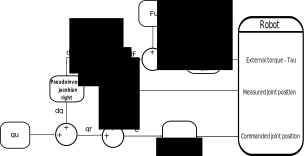
\includegraphics[width=0.75\linewidth]{Pictures/Scheme_Compliance.png}
	\caption{Force compliance block scheme}
	\label{fig:ComplianceBlockScheme}
\end{figure}\\
The external torque of each joint is read and computed to Cartesian forces ($Fm$) with the pseudo-inverse of the Jacobian computed from the last position. This actual Cartesian force is compared with the required force ($Fu$) which can be predefined. The difference is the extra force that the robot should apply. This can be done by giving an extra Cartesian displacement ($\mathrm{d}X$) which is computed with the stiffness matrix. This Cartesian displacement is then translated in joint displacements ($\mathrm{d}q$) with the pseudo-inverse of the Jacobian. If this is subtracted from the position defined by the trajectory ($qu$), then we get our final required position ($qr$) where the robot should be according to the trajectory and the force which should be applied.

Between the required position and the current position, there is an error ($e$). This is the distance in joint space that the robot has to move. This error is controlled by a proportional controller which has a proportional parameter for every joint. $Kp$ is thus a vector with dimension 7 (DOF of the robot). These values are dependent on the required stiffness of each joint. So the vector $Kp$ is dependent on the stiffness matrix. The dependency is just linear scaled.

The controlled value is then added to the current value and commanded to the robot via the low-level joint position controller (see further)~\cite{ComplianceController}.

What is described here, is called admittance control. This means that force is read, and that the desired position is calculated with a specific admittance (reciprocal of the stiffness). So we have an inner position loop which runs at a high frequency and an outer torque loop which shapes the admittance. 

\section{ROS}
For programming the robot, I used ROS~ \cite{ROSTopology} on Linux Ubuntu 16.04 LTS. ROS is a robot operating system that functions as a middleware. ROS abstracts the hardware of a particular robot. The robot functionalities are available to the application program by a unix-like message passing mechanism. ROS is enriched by many libraries and tools to build up the robot software in a modular way and to control robotic components from a PC. With this software, it is possible to let different devices communicate very easily with each other. The codes can be written in different languages and still work together with each other by using topics and services (see further). There are many versions of ROS but I used the Kinetic version as it is one of the newest versions.

\subsection{Nodes}
The whole ROS system consists of a number of independent nodes which works together. A node is just a piece of raw code in C++, Python, \ldots that contains the code to manipulate a certain component like robot actuators or robot sensors. This code is executable and thus consists of a main function.

\subsection{Topics}
Different nodes can communicate with each other via topics, which can be seen as communication channels between the nodes. A node can publish data in the form of messages on a topic. A node can also subscribe messages to a topic.

Publishing means that a node sends data over the topic. Subscribing means that a node reads data from a topic. A message is actually just a data type like int or float but a bit more complex. Every message has a specific msg-file where its data type is described. A message file of the type sensor\textunderscore msgs/JointState that per example is sent over the topic /r1/joint\textunderscore states looks like this:
\begin{verbatim}
std_msgs/Header header
  uint32 seq
  time stamp
  string frame_id
string[] name
float64[] position
float64[] velocity
float64[] effort
\end{verbatim}
You can see that these messages are just a collection of basic programming types like int's, float's, strings, \ldots which are given other names. The principle of publishing and subscribing by topics is shown in Figure \ref{fig:NodeROS}.
\begin{figure}[!ht]
	\centering
	\includegraphics[width=0.75\linewidth, height=4cm]{Pictures/Node_ROS.png}
	\caption{ROS Topic}
	\label{fig:NodeROS}
\end{figure}
In this case, it can be per example the robot that publishes the message with his actual joint positions, velocities, and efforts (torques). There can then be another node, like per example an application, which can subscribe the message to the same topic and can use the information.

\subsection{Services}\label{Services}
This way of communicating by sending messages over topics is just a unidirectional way of communication. You can either send or receive. Another part of ROS are the rosservices. These services make it possible to have a request and response communication. A service like 'switch\textunderscore controllers' can be called to execute a request and receive a response. These services also have types, like the message types on the topics, which are described by srv-files. These service types are really alike to the message types but now consist of two parts: the request part and the response part. An example of the srv-file of the service 'switch\textunderscore controllers' looks like this:
\begin{verbatim}
string[] start_controllers
string[] stop_controllers
int32 strictness
int32 BEST_EFFORT=1
int32 STRICT=2
---
bool ok
\end{verbatim}
The upper part is the type of the request and the lower part is the type of the response. Service communication is shown in Figure \ref{fig:ROSService}.
\begin{figure}[!ht]
	\centering
	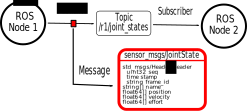
\includegraphics[width=0.75\linewidth, height=4cm]{Pictures/Service_ROS.png}
	\caption{ROS Service}
	\label{fig:ROSService}
\end{figure}
\newpage

\subsection{Master}
This whole traffic system is controlled by the ROS master. This master acts as a name service that controls all the nodes and helps them to find each other by acting like a DNS-server. It provides name registration and lookup for all the nodes, topics and services. The master also acts as a parameter server which keeps track of all the parameters loaded into the nodes. It controls the publishing and subscribing of all the nodes. This whole topology is shown in Figure \ref{fig:ROSTopology}.

\begin{figure}[!ht]
	\centering
	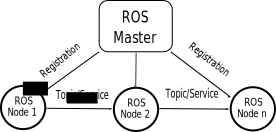
\includegraphics[width=0.75\linewidth, height=6cm]{Pictures/Scheme_ROS.png}
	\caption{ROS Topology}
	\label{fig:ROSTopology}
\end{figure}

In reality, there are a lot of nodes which works together and communicate with each other via the topics and services. If the real robot is started and an application is running on the robot, then we get an nice cooperation between a bunch of nodes which are all managed by the rosmaster. It can be useful to see how all these nodes work together and how they are really bonded with each other. For this, a graphical tool can be used which shows the whole network of nodes which are running during the operation of the robot. This is shown in Figure \ref{fig:GraphicalView}.

\begin{figure}[!ht]
	\centering
		\includegraphics[width=0.75\linewidth]{Pictures/GraphicalView.png}
		\caption{Graphical view of node communication}
	\label{fig:GraphicalView}
\end{figure}

\section{Catkin workspace}
\subsection{Workspace}
So with ROS, all the separate executable code files can be linked by the master and work together to make the robot running. Also important is that this code is well organized so that it is easy for programmers to navigate into the code and to do adaptations. For this purpose, the catkin~\cite{Catkin} workspace is used as a build system for ROS. The principle is that all the code is split up into packages and placed into a workspace. These packages contain all the code that is needed for our system to work and they are located in the source file of our workspace. The fact that we combine all the packages that we need into one workspace makes it possible to compile everything at once and to build the whole code up so that everything works together.

For every part of the system, there is a package. For my applications I use per example a package which contains the code for controlling the robot hand (reflex\textunderscore ros\textunderscore pkg), one to control the industrial gripper (papouch), one for controlling the robot (iiwa\textunderscore fri), one to be able to command the robot (capek\textunderscore testbed), one to use the control manager (ros\textunderscore control) and my own package which contains all the applications (capek\textunderscore robot\textunderscore applications\textunderscore mdr).
All the used packages which are situated in my catkin workspace are shown in Figure \ref{fig:CatkinPackages}.\\
\begin{figure}[!ht]
	\centering
		\includegraphics[width=\linewidth]{Pictures/CatkinPackages.png}
		\caption{Workspace packages}
	\label{fig:CatkinPackages}
\end{figure}\\
These are all the packages that are in my catkin workspace and that thus can be compiled together. Now I am going to explain how a basic package looks like using my own application package.

\subsection{Catkin package}
Every basic package consists of a source folder 'src' which contains executable files (nodes), so these are the programs which can be executed to command the robot. This can be programmed in C++, Python, \ldots In my case, these executables are my applications.

A basic package also contains a package.xml file. This file just gives some more information about the package like the name of the package, authors, dependencies \ldots

And at last, the package consists of a CMakeList.txt file. This file is the input to the package build system ‘Cmake’ which builds the packages and thus compiles everything. This CmakeList.txt file tells the build system how to build the code. It also describes which libraries or other packages are needed to make the current package working. And it describes which code files in the source directory are executable.
So also my package that I made for the applications is constructed like this. It can easily be implemented into other packages. The content of my package is shown in Figures \ref{fig:ApplicationPackageFile} , \ref{fig:ApplicationPackage} and \ref{fig:ContentSRC}.

\begin{figure}[!ht]
	\centering
	\includegraphics[width=3cm]{Pictures/MyPackageFile.png}
	\caption{Application package}
	\label{fig:ApplicationPackageFile}
\end{figure}

\begin{figure}[!ht]
	\centering
	\includegraphics[width=0.75\linewidth]{Pictures/MyPackage.png}
	\caption{Contents of application package}
	\label{fig:ApplicationPackage}
\end{figure}

\begin{figure}[!ht]
	\centering
	\includegraphics[width=0.75\linewidth]{Pictures/ContentSRC.png}
	\caption{Contents of source file}
	\label{fig:ContentSRC}
\end{figure}
\newpage

\subsection{Package.xml-file}
The package.xml-file of my package looks like the following:
\begin{verbatim}
<package format="2">

    <name>capek_robot_applications_mdr</name>
    <version>1.0.0</version>
    <description>
        Applications for robot Capek
    </description>
    <maintainer email="derycmat@fel.cvut.cz">Matthias De Ryck</maintainer>
    <license>BSD</license>

    <buildtool_depend>catkin</buildtool_depend>

    <depend>capek_robot</depend>
    <depend>reflex_msgs</depend>
    <depend>roscpp</depend>
    <depend>controller_manager_msgs</depend>
    <depend>std_srvs</depend>
    <depend>sensor_msgs</depend>
    <depend>iiwa_kinematic</depend>
    <depend>papouch_ros</depend>
</package>
\end{verbatim}
This file only consists of some information about the package. The package format is set to two. This is the required format for new packages. Then there is the name of the package, the version, a description and some details about the author of the package. Further, there is also the software license under which the code is released. In this case, it is BSD (Berkeley Software Distribution)\footnote{https://nl.wikipedia.org/wiki/BSD-licentie}. The requirements set by this license is just that the name of the author and the license need to be mentioned.

In the end, there are also the dependencies on which the package relies on.
In this case, catkin is used as a build tool for all our packages.
So the catkin package is added as our build dependency.\\
Dependencies are packages where our code is dependent on. The code needs the packages to function because it needs other functions and methods defined in these packages.
\begin{easylist}
& Capek\textunderscore robot package is needed to control the robot
& Reflex\textunderscore msgs package contains all the message types needed to control the robot hand & Roscpp package is needed as I programmed in C++. This package contains some libraries and tools for C++
& Papouch\textunderscore ros package contains code to control the industrial gripper
& Other packages are added to make my package work
\end{easylist}
\newpage

\subsection{CMakeList.txt-file}
The CmakeList.txt-file of my package looks like the following:
\begin{verbatim}
cmake_minimum_required(VERSION 2.8.3)
project(capek_robot_applications_mdr)
add_definitions(-std=c++11)

find_package(catkin REQUIRED
  capek_robot
  reflex_msgs
  roscpp
  controller_manager_msgs
  std_srvs
  sensor_msgs
  iiwa_kinematic
  papouch_ros
)

catkin_package()

include_directories(include ${catkin_INCLUDE_DIRS})

add_executable(applicationA_pushing_with_balloon src
applicationA_pushing_with_balloon.cpp)
target_link_libraries(applicationA_pushing_with_balloon ${catkin_LIBRARIES})

add_executable(applicationB_scratching src/applicationB_scratching.cpp)
target_link_libraries(applicationB_scratching ${catkin_LIBRARIES})

add_executable(applicationC_third_hand src/applicationC_third_hand.cpp)
target_link_libraries(applicationC_third_hand ${catkin_LIBRARIES})

add_executable(applicationD_take_object src/applicationD_take_object.cpp)
target_link_libraries(applicationD_take_object ${catkin_LIBRARIES})
\end{verbatim}
The whole package is built based on this file. The file consists of the minimum required version of our building tool, the name of the project/package, and the version of C++ we want to compile in. Next, there are all the dependency packages which should be found by the building tool Cmake. These are the same as in our Package.xml-file. 

Then, of course, our catkin\textunderscore package that we need as our building dependency is defined.

And at the end, all the executable files are added so that the Cmake builder knows which code scripts can be executed. The executables are added and linked to the catkin library.

\section{KUKA LBR iiwa}
The force compliant robot I used is a KUKA LBR iiwa robot with a maximum load of 7 kg and a reaching distance of 800 mm~\cite{KUKALBRiiwa}. This robot has seven rotational joints and thus seven DOF. You can see the robot in Figure \ref{fig:KUKALBRiiwa}. This is a lightweight robot that implements the force compliance by using a torque sensor in each joint. The robot can be controlled by a bunch of controllers which are explained further. These controllers are constantly reading the position (q\textunderscore out) of the joints and the joint torques (tau\textunderscore out) from the servo actuators. This information is gained by the encoders on the robot. Here I am going to repeat that this ability to read torques from the robot is the base of the force compliance. These read torques can be used to do force control. Depending on what mode the robot is operating, joint position (q\textunderscore in) or joint torque (tau\textunderscore in) commands can be given to the servo actuators. Commanding both positions and torques to the robot is impossible. Figure~\ref{fig:KUKAInputsOutputs} shows the inputs and outputs of the robot.

\begin{figure}[!ht]
	\centering
	\includegraphics[width=0.85\linewidth]{Pictures/KUKA_LBRiiwa.png}
	\caption{KUKA LBR iiwa 7kg}
	\label{fig:KUKALBRiiwa}
\end{figure}

\begin{figure}[!ht]
	\centering
	\includegraphics[width=0.25\linewidth]{Pictures/Scheme_KUKA.png}
	\caption{KUKA inputs / outputs}
	\label{fig:KUKAInputsOutputs}
\end{figure}

\section{Grippers}
\subsection{Righthand Robotics robot hand}\label{Robothand}
The ReFlex TakkTile hand of Righthand Robotics~\cite{RighthandRobotics} is a robot hand with three fingers consisting of nine tactile sensors per finger. So force feedback is present. The hand has four motors. Three for each finger and one for a preshape between two fingers. The control of the fingers happens with a wire that runs from the base of the finger (motor) till the top. It is possible to give position, velocity and force commands. To control the hand I made use of the 'reflex\textunderscore ros\textunderscore pkg' which can be downloaded from gitlab:
\url{https://github.com/RightHandRobotics/reflex-ros-pkg.git}.
The hand is controlled via Ethernet. A picture of this hand is shown in Figure \ref{fig:ReflexTakktileHand}.
\begin{figure}[!ht]
	\centering
	\includegraphics[width=5cm]{Pictures/ReflexTakktileHand.png}
	\caption{ReFlex TakkTile hand}
	\label{fig:ReflexTakktileHand}
\end{figure}

\subsection{Schunk industrial robot gripper}\label{Schunk}
This electrical parallel 2-finger gripper is from Schunk~\cite{SchunkGripper}. It is an industrial gripper which can handle small objects. It uses a separate power supply and is controlled via USB or Ethernet. To control the hand I made use of the 'papouch'-package which can be downloaded from gitlab:
\url{http://gitlab.ciirc.cvut.cz/b635/papouch.git}.\\
It is a binary gripper so it can only open or close. A figure is shown in Figure \ref{fig:SchunkGripper}.
\begin{figure}[!ht]
	\centering
	\includegraphics[width=3cm, height=6cm]{Pictures/SchunkGripper.jpg}
	\caption{Schunk industrial robot gripper}
	\label{fig:SchunkGripper}
\end{figure}

\chapter{Literature study}
In this chapter, I am going to talk about the real-time and non-real time control of the robot. These are lower levels of programming. My thesis is situated in the applications which are the highest level of programming. But nevertheless, to work on this level and to be aware of what you are doing, it is also really important to know what is behind the applications. So for that reason, I am going to spend some pages on how the robot is controlled.
\section{Controlling the robot}
\subsection{Configuration of the robot lab}
Before I go into the control of the robots I am going to show first very briefly how the robot configuration was set up in the lab where I worked. The configuration can be seen in Figure \ref{fig:Configuration}. There are two robots which are connected to the KUKA robot controller KRC which controls the communication. These have Windows embedded and are programmed in Java via the KUKA Line interface (KLI). They are both connected to the switch via the KUKA Option Network interface (KONI)\footnote{For more information about KUKA KLI and KONI, please visit the KUKA website www.kuka.com}. In addition, a remote PC named 'CapekPc0' is also connected to the switch. This PC is used as a remote PC with an RT-kernel running on it. Without this RT-kernel all user threads in the operating system would have the same priority. Which can have as a consequence that some tasks can block the communication loop.  The switch is in sequence connected to the wall. Every device has its own static IP-address. Users can connect to the remote PC via DHCP and run their applications.\cite{VladimirPPT}
\begin{figure}[!ht]
	\centering
	\includegraphics[width=0.50\linewidth]{Pictures/capek.pdf}
	\caption{Lab configuration}
	\label{fig:Configuration}
\end{figure}
\newpage
\subsection{Lowest level controller}
The KUKA LBR iiwa robot is controlled by the KUKA Robot Controller (KRC)  \cite{ROSControl} which has Windows embedded and is programmed in Java. With this low-level controller, it is possible to control the robot in two different ways:
\begin{easylist}
& There is either the position controller that sends the computed required position of the joints every 100 times per second to the robot.
& Or either the effort controller which sends the required torque of the joints every 200 times per second to the robot.
\end{easylist}
If the robot does not get the correct information within the required cycle time, it goes in a stop. The controller uses most of the time a PID-controller to control these parameters like position and torque. Set points are imported from the higher level controllers (see further).\\ There is also a joint state controller which gives us the actual robot joint states like joint positions and joint torques. This is our input from the robot that can be used for controlling and for applications.\\There can be switched between the position and effort controller only offline. This is because there are different Java applications needed to be running on the KUKA computers for each control mode. This low-level control is of course real-time. This means that the control loop runs at 100~Hz and thus that there is a new computation and command every 10~ms. The input (only positions in the case of the figure) and output flow to/from the robot is shown in Figure \ref{fig:RobotLowLevelController}.
\begin{figure}[!ht]
	\centering
	\includegraphics[width=0.50\linewidth]{Pictures/Scheme_LowLevelController.png}
	\caption{Low level control}
	\label{fig:RobotLowLevelController}
\end{figure}
\newpage

\subsection{Hardware interface}\label{HardwareInterface}
The output and input of the controllers are positions or torques. But the real robot does not understand this information. The actuators can only be moved with a certain current. Also the output of the encoders is a current. So between the real robot and the controllers, there is need of an interface which translates the values in the program code to real usable values like current.\\For this purpose, the robot hardware interface 'KukaHW' is used, which is actually a software representation of the real robot. It can be seen as an abstraction of the real hardware. This hardware interface is actually a combination of resources. A resource is just something that can be controlled like a joint or also a sensor. The robot it selfs is then a combination of hardware interfaces.\\
Inside this KukaHW there are some aspects taken into account. Per example joint limits. For this, the package joint\textunderscore limits\textunderscore interface is used. It contains data structures to represent joint limits so that the robot is prevented to exceed them. Also the transmission between the servo motors and the joints themselves are taken into account. Joint torques in the robot can be converted to motor torques via some mechanical gearing. The software has to be aware of this an has to recalculate the new values with respect to this transmission.\\
The communication between this hardware abstraction and the real robot hardware goes via FRI through Ethernet. FRI is just an interface that allows the software to communicate with the real robot hardware. In this FRI, the program code is translated to current.\\ The communication between the hardware abstraction and the low-level controller happens via an extra hardware resource interface layer. There are some different types of interfaces which can be used depending on the kind of controller that is used. There are two main groups: There is the joint state interface which reads the joint states in radians from the hardware abstraction. And there is the joint command interface which consists of a joint position/velocity/effort interface. These interfaces give the commands to the hardware abstraction. The kind of interface which should be used is dependent on the type of controller which is used. Per example, if the joint position controller is used, then we need the position joint hardware interface.\\
A visualization of the situation of this hardware interface in the total system is shown in Figure \ref{fig:HardwareInterface}.
\begin{figure}[!ht]
	\centering
	\includegraphics[width=\linewidth]{Pictures/Scheme_HardwareInterface.png}
	\caption{Hardware interface}
	\label{fig:HardwareInterface}
\end{figure}
\newpage

\subsection{Higher level RT-controller}\label{HighLevelControllers}
Next to the lowest level controllers, there are some controllers on a higher level which are programmed as nodes into ROS and run in the real time kernel on another machine than the KUKA controller called capekPc0. These controllers actually control the low-level KUKA controller. The higher level control loop is still real-time and uses an update() command to call the controller (see later). Some types of higher level controllers are:
\begin{easylist}
& effort\textunderscore controller
& position\textunderscore controller
& velocity\textunderscore controller
& trajectory\textunderscore controller: has a sequence of positions as input.
& gravity compensation controller: Lets the robot move in the applied force direction except for gravity force.
& compliance controller: Lets the robot acting like a spring. It is also possible to let the robot apply a constant force in a certain direction.
\end{easylist}
The first four controllers are implemented by ROS. The code for these controllers is available in the ros\textunderscore control-package.\\
The last two controllers are custom controllers developed by the researchers from the Department of Cybernetics and Machine Perception at CTU. I already explained their working principle in Section \ref{ComplianceFunctions}. A visualization of the situation of these controllers in the whole system is shown in Figure \ref{fig:HigherLevelControl}
\begin{figure}[!ht]
	\centering
	\includegraphics[width=\linewidth]{Pictures/Scheme_HighLevelControl.png}
	\caption{Higher level RT-control}
	\label{fig:HigherLevelControl}
\end{figure}
\newpage

\subsubsection{Controller functions}
Here I am going to explain which functions these high-level controllers have and how they are implemented in the real control loop.\\
A basic controller has included the following functions:
\begin{easylist}
& Init(): Looks if the amount of joints in the software matches with the number of real joints on the robot. All the joints in the software are linked to the hardware resources. Here are also some parameters set up like maximum torque or a stiffness matrix.
& Stop(): Cancels all the goals. This is to prevent the robot from moving suddenly while starting the controller again afterwards.
& Start(): Puts every command parameter like position or velocity to a semantic zero.
& Update(): Compute the next position depending on the previous position and torque.
\end{easylist}
The control loop looks like this sequence:
\begin{easylist}
& Read the current state from the hardware
& Transform parameters from actuator to joint state (transmission)
& Update(): Compute the next position depending on the previous position
& Joint limits enforcing
& Transform parameters from joint to actuator command (transmission)
& Write new commands to the hardware
\end{easylist}

In Section \ref{HardwareInterface} about the hardware interface, I already noticed the joint limits and transmissions. A bit more about the joint limits enforcing here. This is the last way of defense before the command goes to the hardware. This under the moto that controllers should not be trusted. It puts some limits to prevent that the joint exceeds his position or velocity limits. A good graph of this behavior is shown in Figure \ref{fig:JointLimitsInterface}.
\begin{figure}[!ht]
	\centering
	\includegraphics[width=0.75\linewidth]{Pictures/JointLimitsEnforce.png}
	\caption{Joint limits enforcing}
	\label{fig:JointLimitsInterface}
\end{figure}
\\
There is also something called the E-stop. This is a procedure that each controller follows after an emergency stop. After such a stop the controllers need to be reset. This is done by calling the stop function first to reset all goals. Then start again. And finally update. This whole procedure can be done in one control cycle.

\subsubsection{Controller manager}
All these higher level controllers need to be managed. This happens by the ROS controller manager which has two main tasks. The first task is the controller lifecycle management. This takes care of loading, unloading, start, stop and switch controllers. A second task is the controller resource management which keeps track of all the resources available like joints and sensors. The manager also has a list of loaded controllers and their type.\\
The needed controllers are loaded when the robot is started. There can be specified which of the loaded controllers already has to start from the beginning.\\
To switch the controllers, a special function is used that can stop a bunch of controllers and start the other needed controllers in one single control cycle. I used it also in my applications where I used the method 'switch\textunderscore controllers(int controller\textunderscore mode)' which I explain in Section \ref{SwitchControllers}. 
It makes use of a rosservice that uses a request type that contains the names of the controllers to stop and the controllers to start.\\ The principle of the control manager is shown in Figure \ref{fig:ControllerManager}.
\begin{figure}[!ht]
	\centering
	\includegraphics[width=0.75\linewidth]{Pictures/Scheme_ControllerManager.png}
	\caption{Controller manager}
	\label{fig:ControllerManager}
\end{figure}\\
So this was the explanation of the RT-part of the robot control. The last part is the NRT-part where the applications are situated. This was my area to work on. But like I already mentioned in the introduction of this chapter, to work on this highest level of programming, a good understanding of what is below is needed. So now that we know how the real-time control of the robot works, we can have a look at how the applications are able to command the robot.
\newpage

\subsection{Higher level NRT-thread}
Next to the real-time part which I explained before, there is also the non-real time part. This part runs in a thread which is separated from the RT-thread. The RT-thread runs at a frequency of 100~Hz while the NRT-thread can run at a lower frequency. These two are separated to prevent a too dense communication travel on one data line. The real-time part is really required to give commands every 10~ms. So this data cannot be disturbed by data which does not need to be transferred that fast. This thread is implemented by adding the 'spinner'-command in our code which I am going to explain later.\\
This NRT-part consists of interfaces according to the loaded controller. These interfaces take care of the communication between the applications and the RT-thread and consists of ros topics, ros services, \ldots The applications can subscribe joint states from the /joint\textunderscore states topic to get all the actual efforts, positions velocities, \ldots These parameters can then be used in the programming logic to build up an application.\\
To send required positions, efforts, trajectories, etc to the controllers, the application uses the NRT-interfaces like MoveIt!\footnote{For more information of what MoveIt! exactly is, see their web page on https://moveit.ros.org/}. Which works between the application and the controller. MoveIt can translate an in the application defined trajectory to a sequence of required points and send it to the RT-controller. There exist also other interfaces like this for other types of applications.
The visualization of the communication of RT- and NRT threads is shown in Figure \ref{fig:DataFlowROS}.
\begin{figure}[!ht]
	\centering
	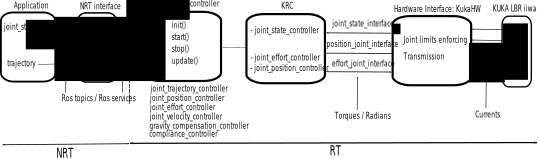
\includegraphics[width=\linewidth]{Pictures/Scheme_NRT.png}
	\caption{RT next to NRT}
	\label{fig:DataFlowROS}
\end{figure}
\newpage

\chapter{Explanation of the code}
Before I go to the applications I am going to explain some important code-related topics which need to be understood before we go to the applications. I am going to explain how the robot is moved using the code and also how the grippers are controlled using the C++ code.\\
For everything that is related to ROS, I used the ROS website \cite{ROS}.

\section{Commanding the robot}
\subsection{Robot commander}\label{RobotCommander}
To command the robot, a class 'CapekRobotCommander' is used. It was written by PhD candidate Vladim\' ir Petr\' ik. This class has several functions to control the robot. It is a bridge between the application level and the higher control level (see chapter 3). At the beginning of every application, this robot commander is declared as follows:
\begin{verbatim}
CapekRobotCommander crc(crc.GROUP_R1_ARM);
\end{verbatim}
An object of the class called 'crc' is made. As an argument, the robot arm we want to command is passed. In this case, robot arm 'R1' is used.
\subsection{Moving in joint space}\label{MovingJoint}
In joint space, the robot is commanded by giving values for each actuator in radians. This can be done using the above mentioned 'CapekRobotCommander'-class. If the robot has to move to a certain position defined by joint positions, then this can be done as follows:\\
A variable 'state' of the type 'robot\textunderscore state::RobotState' is declared. This contains memory for the joint states. The current joint values are assigned to the variable using the CapekRobotCommander crc object. 'getCurrentState()' is one of its methods. Then all the variables are set to 0.0 radians using the setToDefaultValues() method. Next, every required joint position is defined in radians for each joint. '-M\textunderscore PI\textunderscore 2' means that joint one moves 90 degrees (PI / 2) in negative direction.
\begin{verbatim}
robot_state::RobotState state = *crc.getCurrentState();
state.setToDefaultValues();
state.setVariablePosition("r1_joint_1", -M_PI_2);
state.setVariablePosition("r1_joint_2", M_PI/6.0);
state.setVariablePosition("r1_joint_3", 0.0);
state.setVariablePosition("r1_joint_4", -M_PI/3.0);
state.setVariablePosition("r1_joint_5", 0.0);
state.setVariablePosition("r1_joint_6", M_PI_2);
state.setVariablePosition("r1_joint_7", 0.0);
crc.setJointValueTarget(state);
crc.move()
\end{verbatim}
By using the function setJointValueTarget() from crc, all the set points for the joints are set and executed using the move() function. The robot will then move to the defined position defined in the joint space.

\subsection{Moving in Cartesian space}
Moving the robot in Cartesian space is a bit more difficult. The first step is the same. Also the current joint values are assigned to a variable 'state'.
\begin{verbatim}
robot_state::RobotState state = *crc.getCurrentState();
\end{verbatim}
Next, the global transformation matrix which transforms the base frame through all the joints to the end effector frame 'r1\textunderscore ee' is defined using the current joint state values. Now the exact Cartesian position of the end effector 'r1\textunderscore ee' is known. This matrix is called matrix $A$. If the robot has to move 10~cm in negative $z$-direction, then the  matrix $A$ is multiplied with a translation matrix as shown. Matrix $B$ is obtained. This matrix contains now the desired Cartesian position.
\begin{verbatim}
Eigen::Affine3d A = state.getGlobalLinkTransform("r1_ee");
Eigen::Affine3d B = A * Eigen::Translation3d(0.0, 0.0, -0.10);
\end{verbatim}
For a rotation around one of the Cartesian axes, a similar rotation matrix is used.
The following command rotates around the $X$-axis with 90 degrees in positive direction. Which is from $Y$-axis to $Z$-axis.
\begin{verbatim}
Eigen::Affine3d C = B * Eigen::AngleAxisd(M_PI_2, Eigen::Vector3d::UnitX())
\end{verbatim}
To compute the path, the method computeCartesianPath() is used. It divides the total Cartesian path from current end effector position to position B and further to position C in small pieces dependent on the speed of the robot and the frequency of the control loop. The sequence of Cartesian points is saved into the trajectory data type 'rtraj'. The end effector frame and the arm that has to move are also specified. This movement is then executed using the execute() method. It uses the rtraj.joint\textunderscore trajectory-type which contains the individual joint positions for each Cartesian point.
\begin{verbatim}
moveit_msgs::RobotTrajectory rtraj;
crc.computeCartesianPath(rtraj, {B, C}, "r1_ee", "r1_arm");
crc.execute(rtraj.joint_trajectory);
\end{verbatim}
\section{Commanding the robot hand}
\subsection{Calibration} \label{CalibratingHand}
The calibration is done by services. The first step is to make service messages. In this case, empty messages are used as there is no need to send or receive data.
\begin{verbatim}
std_srvs::Empty cal_fing;
std_srvs::Empty cal_tact;
\end{verbatim}
The service is then called with the name of the service and the messages passed:
\begin{verbatim}
ros::service::call("/reflex_takktile/calibrate_fingers", cal_fing);
ros::service::call("/reflex_takktile/calibrate_tactile", cal_tact);
\end{verbatim}

\subsection{Controlling} \label{ControllingHand}
The hand is controlled using publishers. The position publisher 'pos\textunderscore pub' per example is declared as follows:
\begin{verbatim}
ros::Publisher pos_pub = n.advertise<reflex_msgs::PoseCommand>("/reflex_takktile
/command_position", 1);
\end{verbatim}
The message type is defined between '\textless \textgreater'. The topic name is passed as an argument.\\
There are publishers to publish a position, a velocity, a command (position + velocity) and a force. To publish messages on a topic, first the messages have to be made. As an example I am going to show how a position is commanded.
Therefore a message of the type 'reflex\textunderscore msgs::PoseCommand' has to be made:
\begin{verbatim}
reflex_msgs::PoseCommand pose;
\end{verbatim}
This message looks like this:
\begin{verbatim}
# Position in radians of various motors
float64 f1
float64 f2
float64 f3
float64 preshape
\end{verbatim}
The message is made by defining the required position of each finger (f1, f2 and f3). Also the preshape position between fingers 2 and 3 is defined.
\begin{verbatim}
pose.f1 = 0.0; pose.f2 = 0.0; pose.f3 = 0.0; pose.preshape = 0.0;
\end{verbatim}
Then the message is published:
\begin{verbatim}
pos_pub.publish(pose);
\end{verbatim}
If this would be done once, then the hand would just move a little bit and then return to its original state again because this publishing only takes a few milliseconds. So it is required to keep publishing the message until the required position is reached.
\begin{verbatim}
reflex_msgs::Hand hand_state;

do{
	    pose.f1 = 0.0; pose.f2 = 0.0; pose.f3 = 0.0; pose.preshape = 0.0;
	    pos_pub.publish(pose);
	    msg = ros::topic::waitForMessage<reflex_msgs::Hand>("/reflex_takktile/	
	    hand_state");
	    hand_state = *msg;
	}while(abs(hand_state.motor[0].joint_angle) > 0.1 or
	abs(hand_state.motor[1].joint_angle) > 0.1 or
	abs(hand_state.motor[2].joint_angle) > 0.1);
\end{verbatim}
The do-while-loop keeps going until the position of every finger is reached. As the hand will never reach 0.0 degrees exactly (due to noise on the sensors), I solved it by stopping if an angle smaller then 0.1 is reached. The information is read from the topic '/reflex\textunderscore takktile/hand\textunderscore state':
\begin{verbatim}
msg = ros::topic::waitForMessage<reflex_msgs::Hand>("/reflex_takktile/	hand_state");
hand_state = *msg;
\end{verbatim}
The method waitForMessage\textless 'message type'\textgreater ('topic') reads one message from the topic. The variable hand\textunderscore state.motor[0].joint\textunderscore angle is the angle in radians of finger one. This message type may look a bit difficult. This is because here, a message type is defined using other message types. The variable 'hand\textunderscore state' that is used, is of the type 'reflex\textunderscore msgs::Hand'. This means that in the message folder 'reflex\textunderscore msgs', there is a message file called 'Hand' which defines the message type. This message type looks like this:
\begin{verbatim}
Finger[3] finger      # Pointer = finger[0], Middle = finger[1], Thumb = finger[2]
Motor[4] motor        # Finger 1, Finger 2, Finger 3, and Preshape
\end{verbatim}
The type finger and motor are also message types which are located in the same folder. The message type 'motor' looks like this:
\begin{verbatim}
float64 joint_angle
float64 raw_angle
float64 velocity
float64 load
float64 voltage
int32 temperature
string error_state
\end{verbatim}
Here we have the variable 'joint\textunderscore angle' that we want. So if the value of the joint position in radians of finger one is needed, the declared variable hand\textunderscore state of the type 'reflex\textunderscore msgs::Hand' is called and is asked for its variable 'motor[0]', which is motor of finger one, using '.motor[0]'. And to obtain the joint angle of this motor, his variable joint\textunderscore angle is called using '.joint\textunderscore angle'. So in total this becomes:
\begin{verbatim}
hand_state.motor[0].joint_angle
\end{verbatim}
\newpage

\section{Commanding the industrial gripper}\label{CommandingGripper}
This gripper can easily be controlled using the code because the only two commands that can be given are open and close. To transfer these commands to the gripper, a service is used. The first task is to make a service message. This message is of the type 'papouch\textunderscore ros::WriteIO' and looks like this:
\begin{verbatim}
int8[] channel
int8[] state
---
bool retval
\end{verbatim}
Only channel one is used to open and channel two to close. I made the message as follows:
\begin{verbatim}
papouch_ros::WriteIO open_gripper;
	papouch_ros::WriteIO close_gripper;

	std::vector<int8_t> channel_open;
	channel_open.resize(2);
	channel_open[0] = 2; #Channel 2
	channel_open[1] = 1; #Channel 1

	std::vector<int8_t> state_open;
	state_open.resize(2);
	state_open[0] = 0;	#Chanel 2 has state 0 to open
	state_open[1] = 1;	#Chanel 1 has state 1 to open

	std::vector<int8_t> channel_close;
	channel_close.resize(2);
	channel_close[0] = 1;	#Channel 1
	channel_close[1] = 2;	#Channel 2

	std::vector<int8_t> state_close;
	state_close.resize(2);
	state_close[0] = 0;	#Chanel 1 has state 0 to close
	state_close[1] = 1;	#Chanel 2 has state 1 to close

	open_gripper.request.channel = channel_open;
	open_gripper.request.state = state_open;
	close_gripper.request.channel = channel_close;
	close_gripper.request.state = state_close;
\end{verbatim}
Two messages 'open\textunderscore gripper' and 'close\textunderscore gripper' are declared. Then four vectors are made with the data. Two (channel and state) for each message. These vectors are then assigned to the messages. The gripper can then easily being opened and closed by calling the service "/write\textunderscore io" giving it the constructed messages:
\begin{verbatim}
ros::service::call("/write_io", open_gripper)
ros::service::call("/write_io", close_gripper)
\end{verbatim}

\chapter{Applications}
In cooperation with the whole department, we came to the following four applications which shows all of the implemented functions mentioned in paragraph \ref{ComplianceFunctions}. The applications are meant to show a nice and fluent interaction with humans. The purpose is to make companies warm to use this new technology, and to show them that the whole setup is safe an can be easily implemented in every situation. For the programmation of the applications, I used the packages that already existed and were developed by PhD candidate Vladim\' ir Petr\' ik. I programmed the code in C++ to make it uniform with the already written pieces. The full code for each application can be found in the appendix.\\
Sometimes I am going to refer to joint numbers of the robot, these numbering of joints is showed in Figure \ref{fig:KUKALBRiiwa}.

\section{Issue about the used grippers}
Initially, it was the purpose for me to work with the robot hand of Righthand robotics mentioned in Section \ref{Robothand} for all four applications. Unfortunately, there went something wrong with the hand which caused that I had to look for a second option which is the industrial gripper mentioned in Section \ref{Schunk}. I did research on them both so I was able to control them both and implement them in my applications. I could do this before the hand was broken. But in the end, I could only do experiments with the industrial gripper. So the codes which are added in the appendices and which are the codes of my final applications,  are written using this gripper or without a gripper. In the further sections, I am going to explain the sequence of every application using the industrial gripper. Sometimes I will refer to the robot hand and explain how this hand would have been implemented in the code.
\newpage

\section{Structure of the code} \label{Structure}
To make the applications consistent, they are made up in the same way with the same start and end procedure. They are written in one single piece of code (one file) to make it as a nice and clean unit. Every application starts with the following sequence:
\begin{easylist}
& Including packages: In the code, I use methods and functions that are already implemented in other packages. In this part, all the packages that are needed are implemented.
& Implementing all the self-written functions. These are functions that are used in the sequence of the code and are placed in a separate function to make the code easier to read.
& The main function: This is the function where the code sequence is started. From here, all the self-written functions mentioned above are called.
\end{easylist}

The main function contains the main sequence of the process. This sequence is also made in a consistent way for all the applications. The sequence is as follows:
\begin{easylist}
& Some information about the application which is started is given
& Initializing the node
& Declare the robot commander and some publishers or services
& Set controller mode to the trajectory mode. This to be sure that the robot is not in another mode caused by a previous application which ended badly.
& Move to the initial position
& Specific sequence of the application
& Set controller mode to the trajectory mode
& Move to the initial position
& End of the application
\end{easylist}

In the following sections, all of the above general functions/parts which apply for every application are explained.

\subsection{Include packages}
In every application, I include the ros.h file and the CapekRobotCommander.h file. The ros package is needed to make a rosnode from the code and make it executable and callable in the ROS-topology. The CapekRobotCommander is used to command the robot and thus lets him make trajectories. It is a bridge between the application level and the higher level controllers. I also include a package which includes the message file to switch the controllers. When torques have to be read, there is also a package needed which contains the joint state message. When the industrial gripper is used, the package which contains the service message file to control it is also included.
\begin{verbatim}
#include <ros/ros.h>
#include <capek_robot/CapekRobotCommander.h>

#include <controller_manager_msgs/SwitchController.h>

#include <sensor_msgs/JointState.h>
#include <papouch_ros/WriteIO.h>
\end{verbatim}

\subsection{General self-written functions}
These are functions that are used in every application and called from the main function. This to make an abstraction of the functions and to make the code easier to read. The self-written functions which are unique for each application are described in following sections per application.
\subsubsection{Function: switch\textunderscore controllers()}\label{SwitchControllers}
In Section \ref{HighLevelControllers}, I explained some of the used controllers that are used in the higher level control of the robot. I use the trajectory controller to let the robot make certain trajectories, the gravity compensation controller to be able to move the robot by hand, and the compliance controller to show the compliant functions of the robot. It is possible to change between these controllers online. This function makes this possible.
The argument that is passed defines which controllers shall be stopped and which shall be started, using if-else-functions. This is done via a rosservice. First a message 'srv\textunderscore switch' of the type 'controller\textunderscore manager\textunderscore msgs::SwitchController' is made. How this message looks like can be seen in Section \ref{Services}. This message contains the parameters 'strictness', 'start\textunderscore controllers' and 'stop\textunderscore controllers'. Once the message is made depending on the argument, the message is sent over the service '/r1/controller\textunderscore manager/switch\textunderscore controller'.
When the service is called, the controllers are switched. This is done in one single control cycle.
\begin{verbatim}
bool switch_controllers(int controller_mode) {

    	controller_manager_msgs::SwitchController srv_switch;
    	srv_switch.request.strictness =
    	controller_manager_msgs::SwitchController::Request::BEST_EFFORT;
    	
    	if (controller_mode == 0) {
       	srv_switch.request.start_controllers.push_back("trajectory_controller");
       	srv_switch.request.stop_controllers.push_back("compliance_controller");
        srv_switch.request.stop_controllers.push_back("gravity_compensation_controller");
   	 } else if(controller_mode == 2){
        srv_switch.request.start_controllers.push_back("gravity_compensation_controller");
        srv_switch.request.stop_controllers.push_back("compliance_controller");
		        srv_switch.request.stop_controllers.push_back("trajectory_controller");
     } else{
		        srv_switch.request.start_controllers.push_back("compliance_controller");
        srv_switch.request.stop_controllers.push_back("gravity_compensation_controller");
		        srv_switch.request.stop_controllers.push_back("trajectory_controller");
    	}
    	
    	if (!ros::service::call("/r1/controller_manager/switch_controller", srv_switch)) {
       		 ROS_ERROR_STREAM("Cannot switch controllers.");
        	return false;
    	}
    	
    	return true;
}
\end{verbatim}
\newpage

\subsubsection{Function: moveToInitialPosition()}
To make the application consistent, the robot moves always to the initial position first. This is an L-shape position which you can see in Figure \ref{fig:InitialPosition}. The robot is moved using the moveToNamedTarget() method. This is the same as in Section \ref{MovingJoint} but now the variable 'NAMED\textunderscore TARGET\textunderscore L' contains predefined joint states in radians. The execution happens with the move()-command.
\begin{verbatim}
int moveToInitialPosition(CapekRobotCommander &crc){

	    //Move robot to initial position
	    crc.moveToNamedTarget(crc.NAMED_TARGET_L);

	    if (!crc.move()) {
		        ROS_ERROR_STREAM("Cannot move to initial position");
		        return -1;
	    }
	
	    ROS_INFO_STREAM("Moved to initial position");
}
\end{verbatim}
If the robot hand is used, then also this hand goes to an initial position. In this position the robot hand is open. All its fingers are positioned at 60 degrees. This is done like in Section \ref{ControllingHand}. But now a command (position + velocity) is published. The position information is again read from the "/reflex\textunderscore takktile/hand\textunderscore state"-topic.
\begin{verbatim}
//Move hand to initial position
do{
		    pose.f1=M_PI/3.0; pose.f2=M_PI/3.0; pose.f3=M_PI/3.0;
		    velocity.f1=15.0; velocity.f2=15.0; velocity.f3=15.0;
		    command.pose = pose; command.velocity = velocity;
		    command_pub.publish(command);
		    msg = ros::topic::waitForMessage<reflex_msgs::Hand>("/reflex_takktile/hand_state");
		    hand_state = *msg;
}while(hand_state.motor[0].joint_angle < M_PI/3.1 or
 hand_state.motor[1].joint_angle < M_PI/3.1 or
 hand_state.motor[2].joint_angle < M_PI/3.1);
\end{verbatim}
If the industrial gripper is used, then this gripper goes also to an initial position which is open. So just the service is called:
\begin{verbatim}
if (!ros::service::call("/write_io", open_gripper)) {
       		ROS_ERROR_STREAM("Cannot open gripper.");
        return -1;
}
\end{verbatim}
\newpage

\begin{figure}[!ht]
	\centering
	\includegraphics[width=4cm, height=5cm]{Pictures/InitialPosition.jpg}
	\caption{Initial position of the robot}
	\label{fig:InitialPosition}
\end{figure}

\subsubsection{Function: moveHandToDefaultPosition()}
If the robot hand is used, this function is called in almost every application. Before the robot moves to its initial position, the hand first moves to a default position. This to prevent the hand to be in an unknown state caused by a previous application which ended badly. First, the fingers and tactile sensors are calibrated via services like in Section \ref{CalibratingHand}. Then the hand is moved to its default position by publishing a zero degree pose. The publishing keeps going until the required position is reached like in Section \ref{ControllingHand}.
\begin{verbatim}
void moveHandToDefaultPosition(ros::Publisher &pos_pub){

	    //Calibrating hand
	    std_srvs::Empty cal_fing;
	    std_srvs::Empty cal_tact;

	    ros::service::call("/reflex_takktile/calibrate_fingers", cal_fing);
  	 ros::service::call("/reflex_takktile/calibrate_tactile", cal_tact);

	    ROS_INFO_STREAM("Hand is calibrated.");

	    //Move hand to default position
	    do{
		        pose.f1=0.0; pose.f2=0.0; pose.f3=0.0;
		        pos_pub.publish(pose);
		        auto msg = ros::topic::waitForMessage<reflex_msgs::Hand>("/reflex_takktile
		        /hand_state");
		        hand_state = *msg;
		        ROS_INFO_STREAM(hand_state.motor[0].joint_angle);
	    }while(hand_state.motor[0].joint_angle > 0.1 or
	     hand_state.motor[1].joint_angle > 0.1 or
	     hand_state.motor[2].joint_angle > 0.1);

	    ROS_INFO_STREAM("Hand moved to default position");
}
\end{verbatim}
\newpage

\subsection{Main function}
In this section, the general sequence of the main function is explained which is the same for every application.
\subsubsection{Initializing the node}
After a piece of information about the application is given to the user using the ROS\textunderscore INFO\textunderscore STREAM - command, every main function of every application starts with initializing the node. This means that the raw piece of C++ code becomes an executable that can be called and controlled by the rosmaster. With the ros::init() command, the node is initialized and is given a unique name. The master can now register the name. The ros::NodeHandle n command declares a node handle which is used to start and stop the node easily and to assign it a subscriber or publisher. The object spinner lets the node run in a separate NRT-thread than the master. So these are now 2 threads which run in parallel. The thread is started using spinner.start().
\begin{verbatim}
//Initializing the node
	ros::init(argc, argv, "Name of node");
	ros::NodeHandle n;
	ros::AsyncSpinner spinner(2);
	spinner.start();
	ROS_INFO_STREAM("Node initialized");
\end{verbatim}

\subsubsection{Declare robot commander}
To control the robot, the class CapekRobotCommander is used as explained in Section \ref{RobotCommander}. The object always has 'crc' as name. Now, there are some methods like crc.move(), crc.setRobotSpeed(1.0) or crc.stop() which can control the robot. To start the application, the speed is set to 1~m/s.
\begin{verbatim}
//Declare robot commander and publishers
	CapekRobotCommander crc(crc.GROUP_R1_ARM);
	crc.setRobotSpeed(1.0);
\end{verbatim}

\subsubsection{Set controller to trajectory mode}\label{SetController}
Before the robot makes any move, the controller is set to the trajectory controller so the robot is able to move to its initial position. This is done to be sure that the robot is in a well-defined mode and not in any other unknown mode which is still active due to a previous application which ended badly.
The previously described method 'switch\textunderscore controllers(int controller\textunderscore mode)' is used with the argument '0'. Which means that the trajectory controller will be started and all other controllers stopped. If the controller cannot be switched, the service gives a '-1' or 'False' as respond. This exception is caught and the information is sent to the user.
\begin{verbatim}
//Set controller mode to mode 0 (Trajectory mode)
	if (!switch_controllers(0)) {
		    ROS_ERROR_STREAM("Cannot set to mode 0");
		    return -1;
	}
\end{verbatim}

\section{Application A: Pushing the robot with a balloon}
In this application, the robot is literally going to be pushed with a balloon or with a soft object. This application shows that the robot can be handled very smoothly and without a lot of force. If a balloon is used, the deformation of the balloon while pushing the robot is a good indication of the force that is needed to push. For this purpose, the compliance controller is used. With this controller, the robot will act like a spring. I already mentioned this function in paragraph \ref{ComplianceFunctions}. So the robot can be pushed by a balloon and when the applied force reduces to zero, the robot comes back to its initial position. The stiffness of the robot and thus its compliance can be adapted easily.

\subsection{Explanation of the code}
The full code can be found in appendix \ref{Bijlage1}.
The first general parts of the process are explained in Section \ref{Structure}.
After the node is initialized, the CapekRobotCommander is declared, the controller is set to trajectory mode and the robot moved to the initial position, the robot can move to a starting position which you can see in Figure \ref{fig:AStartingPosition}. This is done using the following code:
\begin{verbatim}
int moveToStartPosition(CapekRobotCommander &crc){

	    //Move robot to start position
	    robot_state::RobotState state = *crc.getCurrentState();
	    state.setToDefaultValues();
	    state.setVariablePosition("r1_joint_1", -M_PI_2);
	    state.setVariablePosition("r1_joint_2", M_PI/6.0);
	    state.setVariablePosition("r1_joint_3", 0.0);
	    state.setVariablePosition("r1_joint_4", -M_PI/3.0);
	    state.setVariablePosition("r1_joint_5", 0.0);
	    state.setVariablePosition("r1_joint_6", M_PI_2);
	    state.setVariablePosition("r1_joint_7", 0.0);
	    crc.setJointValueTarget(state);

	    if (!crc.move()) {
		        ROS_ERROR_STREAM("Cannot move to start position");
		        return -1;
	    }

	    ROS_INFO_STREAM("Moved to start position");

}
\end{verbatim}
\newpage
This position is chosen in a way that the robot can easily be pushed with a balloon by a person. As soon as the robot is in this position, the controller is switched to the compliance controller. This is done in the same way is in Section \ref{SetController}. But now argument '3' is given to specify the compliance controller.
\begin{verbatim}
//Set controller mode to mode 3 (Compliance mode)
	if (!switch_controllers(3)) {
		    ROS_ERROR_STREAM("Cannot set to mode 3");
		    return -1;
	}
	
	ROS_INFO_STREAM("Controller mode set to mode 3 (Compliance mode)");
\end{verbatim}
Once this controller is active, it is possible to push the robot with the balloon. The display shows ``Push the robot with the balloon'', ``Press enter when done''. So when enter is pressed, the controller changes to trajectory controller. The robot moves then back to its initial position and the application is ended.
\begin{figure}[!ht]
	\centering
	\includegraphics[width=8cm]{Pictures/AStartingPosition.jpg}
	\caption{Application A: Starting position}
	\label{fig:AStartingPosition}
\end{figure}
\newpage

\section{Application B: Scratching a persons back}
I think there cannot be a closer human-robot interaction than a robot which scratches a persons back. Here the human can really experience how soft the robot can handle. The robot moves to a position from where he starts the scratching. When a button is pressed, the robot starts to execute a predefined path parallel to the persons back. The force perpendicular to the persons back and thus the trajectory that follows the back relief is done by force control. This gives as a result that the person feels a comfortable and constant force applied to his back.

\subsection{Explanation of the code}
The full code can be found in appendix \ref{Bijlage2}.
The first general parts of the process are explained in Section \ref{Structure}.
After the node is initialized, the CapekRobotCommander is declared, the controller is set to trajectory mode and the robot moved to the initial position, the display shows "Press enter to start scratching". When enter is pressed, the robot moves to its starting position which you can see in Figure \ref{fig:BStartingPosition}. This is done using the following code:
\begin{verbatim}
int moveToStartPosition(CapekRobotCommander &crc){

	    //Move robot to start position
	    auto state = *crc.getCurrentState();
	    state.setToDefaultValues();
	    state.setVariablePosition("r1_joint_1", M_PI_2);
	    state.setVariablePosition("r1_joint_2", M_PI/6.0);
	    state.setVariablePosition("r1_joint_3", 0.0);
	    state.setVariablePosition("r1_joint_4", -M_PI/3.0);
	    state.setVariablePosition("r1_joint_5", 0.0);
	    state.setVariablePosition("r1_joint_6", 0.0);
	    state.setVariablePosition("r1_joint_7", 0.0);
	    crc.setJointValueTarget(state);
	    crc.move()
	
	    ROS_INFO_STREAM("Moved to start position");
}
\end{verbatim}
\begin{figure}[!ht]
	\centering
	\includegraphics[width=6cm]{Pictures/BStartPosition.jpg}
	\caption{Application B: Starting position}
	\label{fig:BStartingPosition}
\end{figure}
\newpage

Afterwards, the following is printed: ``Press enter when person is ready''. When enter is pressed the function 'scratch()' is called. This function looks like the following:
\begin{verbatim}
void scratch(CapekRobotCommander &crc){

	    //Move towards person. If there is no person, application will end.
	    //If there is a person, scratching starts
	    ROS_INFO_STREAM("Detect person");

	    CapekRobotCommander::Plan plan;
	    robot_state::RobotState state = *crc.getCurrentState();
	    Eigen::Affine3d A = state.getGlobalLinkTransform("r1_ee");
	    Eigen::Affine3d B = A * Eigen::Translation3d(0.0, 0.0, +0.1);

	    moveit_msgs::RobotTrajectory rtraj;
	    crc.computeCartesianPath(rtraj, {B}, "r1_ee", "r1_arm");
	    crc.plan(plan);
	    plan.trajectory_ = rtraj;
	    crc.showTrajectory(plan);
	    crc.setRobotSpeed(0.2);

	    //This command computes trajecory without waiting till it's done =>
	    //can be stopped by crc.stop()
	    crc.asyncExecute(plan);

	    getForceMeasurements();

	    if(effort[1] < -1.0){
		        ROS_INFO_STREAM("Person detected, start scratching path.");
		        crc.stop();

		        //Set controller mode to mode 3 (Compliance mode)
		        if (!switch_controllers(3)) {
			            ROS_ERROR_STREAM("Cannot set to mode 3");
			            return -1;
		        }

		        ROS_INFO_STREAM("Controller mode set to mode 3 (Compliance mode)");
		        computeScratchPath(crc);
	    }
	    else{
		        ROS_INFO_STREAM("No person to scratch");
	    }
	
	    crc.setRobotSpeed(1.0);
	
}
\end{verbatim}
The robot moves 10~cm towards the person to detect the person. While executing the path, force measurements are gained using the function getForceMeasurements():
\begin{verbatim}
Eigen::Matrix<double, 7, 1> effort;

void getForceMeasurements(){

	    sensor_msgs::JointState r1_joint_states;

	    do{
		      auto msg = ros::topic::waitForMessage<sensor_msgs::JointState>("/r1/joint_states");
		      r1_joint_states = *msg;
		      for (size_t i = 0; i < effort.size(); ++i) {
        		  effort(i, 0) = r1_joint_states.effort[i];
    		 }
	    }while(r1_joint_states.effort[1] > -1.0 and r1_joint_states.velocity[0] != 0);
}
\end{verbatim}
If the force in joint two, which undergoes the highest torque, exceeds 1~N, then the method stops and the sequence goes back to the 'scratch()' method and ``Person detected, start scratching path.'' appears on the screen. The robot movement stops using crc.stop(). The controller is set to the force compliant mode to apply a constant force perpendicular to the persons back. Finally the scratch path is executed using the computeScratchPath()-function. This function looks like this:
\begin{verbatim}
int computeScratchPath(CapekRobotCommander &crc){

	    ROS_INFO_STREAM("Scratching...");

	    CapekRobotCommander::Plan plan;
	    robot_state::RobotState state = *crc.getCurrentState();
	    Eigen::Affine3d X = state.getGlobalLinkTransform("r1_ee");
	    Eigen::Affine3d A = X * Eigen::Translation3d(0.1, -0.1, 0.0);
	    Eigen::Affine3d B = A * Eigen::Translation3d(0.2, 0.0, 0.0);
	    Eigen::Affine3d C = B * Eigen::Translation3d(0.0, 0.2, 0.0);
	    Eigen::Affine3d D = C * Eigen::Translation3d(0.2, 0.0, 0.0);
	    Eigen::Affine3d E = D * Eigen::Translation3d(0.0, -0.2, 0.0);
	    Eigen::Affine3d F = E * Eigen::Translation3d(-0.4, 0.2, 0.0);
	    Eigen::Affine3d G = F * Eigen::Translation3d(-0.1, -0.1, 0.0);
	
	    moveit_msgs::RobotTrajectory rtraj;

	    crc.computeCartesianPath(rtraj, {A, B, C, D, E, F, G}, "r1_ee", "r1_arm");
	    crc.plan(plan);
	    plan.trajectory_ = rtraj;
	    crc.showTrajectory(plan);
	    crc.execute(plan);
	    ROS_INFO_STREAM("End of scratching");
}
\end{verbatim}
This is just a scratch path defined in Cartesian space. After the path is executed, the controller changes back to trajectory controller and the robot moves to its initial position. The application is ended.\\
When no person was detected in the trajectory of 10~cm. This means that no force of 1~N is exceeded. The getForceMeasurements-function stops because the velocity in joint 1 is zero after the trajectory is ended. ``No person to scratch'' appears on the display and the same end procedure is followed.
\newpage

\section{Application C: Third hand}
Probably everyone already had once a moment while doing a certain job where he wished that he had one more hand to complete the job. Like per example in welding. If you have a vertical surface where you want to weld a piece of metal on, it can become really tricky to do the job fluently. You need a hand for the electrode, a hand for the mask, and then it would be good if your third hand, which you unfortunately do not have, could help you to hold the piece of steel in place. For this purpose, there is this demo where the robot arm can be your third hand. You can guide the robot with your hand to whatever position you like it to be. And then you can let it apply a certain force perpendicular to the steel plate so that it is fixed and you can easily do the job. Afterwards, you can guide the robot back to another position.

\subsection{Explanation of the code}
The full code can be found in appendix \ref{Bijlage3}.
The first general parts of the process are explained in the Section \ref{Structure}.
After the node is initialized, the CapekRobotCommander is declared, the controller is set to trajectory mode and the robot moved to the initial position, the robot moves to a starting position. This position is chosen in a way that the gravity compensation mode can be started. Gravity compensation mode only works when every joint position is larger than ten degrees from its default position. This to avoid singularities during the movement. So the robot moves to a position where this is the case. This position can be seen in Figure \ref{fig:CStartingPosition}. This is done using the following function:
\begin{verbatim}
int moveToStartPosition(CapekRobotCommander &crc){

	    //Move robot to start position
	    auto state = *crc.getCurrentState();
	    state.setToDefaultValues();
	    state.setVariablePosition("r1_joint_1", 0.0);
	    state.setVariablePosition("r1_joint_2", 15.0 * M_PI / 180.0);
	    state.setVariablePosition("r1_joint_3", 0.0);
	    state.setVariablePosition("r1_joint_4", -M_PI_2);
	    state.setVariablePosition("r1_joint_5", 0.0);
	    state.setVariablePosition("r1_joint_6", M_PI_2 - 15.0 * M_PI / 180.0);
	    state.setVariablePosition("r1_joint_7", 0.0);
	    crc.setJointValueTarget(state);
	    crc.move()
	    ROS_INFO_STREAM("Moved to start position");
}
\end{verbatim}
As soon as the robot is in this position, the controller is switched to the gravity compensation controller using argument ``2''. ``Press enter to clamp'' is showed on the display.
\begin{verbatim}
//Set controller mode to mode 2 (Gravity compensation mode)
	if (!switch_controllers(2)) {
		    ROS_INFO_STREAM("Cannot set to mode 2");
		    return -1;
	}
	ROS_INFO_STREAM("Controller mode set to mode 2 (Gravity compensation mode));
\end{verbatim}
From now on there is a loop processing so the user can constantly switch between gravity compensation and trajectory mode by pressing enter. The display also shows: ``Press enter to guide'' or ``Press enter to clamp''. So if the robot is in gravity compensation mode and can thus be guided, then the user can press enter when he wants the robot to clamp an object. When enter is pressed, trajectory mode is activated and the robot tries to clamp the object using the function ``clamp()'':
\begin{verbatim}
int clamp(CapekRobotCommander &crc){
	
	crc.setRobotSpeed(0.1);
	
	//Move towards object. Cycle continues regardless if there is an object or not.
	CapekRobotCommander::Plan plan;

	robot_state::RobotState state = *crc.getCurrentState();
	Eigen::Affine3d A = state.getGlobalLinkTransform("r1_ee");
	Eigen::Affine3d B = A * Eigen::Translation3d(0.0, 0.0, +0.05);

	moveit_msgs::RobotTrajectory rtraj;

	crc.computeCartesianPath(rtraj, {B}, "r1_ee", "r1_arm");

	crc.plan(plan);
	plan.trajectory_ = rtraj;
	crc.showTrajectory(plan);

	//This command computes trajecory without waiting till it's done =>
	//can be stopped by crc.stop()
	crc.asyncExecute(plan);

	getForceMeasurements();

	if(effort[0]>10 or effort[1]>10 or effort[2]>10 or effort[3]>10 or effort[4] > 10){
		    crc.stop();
		    ROS_INFO_STREAM("Object clamped, press enter to stop clamping");
		    	
		    //Set controller mode to mode 3 (Compliance mode)
		    if (!switch_controllers(3)) {
			        ROS_ERROR_STREAM("Cannot set to mode 3");
			        return -1;
		    }
	}
	else{
		    ROS_INFO_STREAM("Object is not clamped");
	}
	crc.setRobotSpeed(1.0);
}
\end{verbatim}
In this function, the robot moves 5~cm towards the object. While the movement is made, the function getForceMeasurements() is called. This function is written as follows:
\begin{verbatim}
Eigen::Matrix<double, 7, 1> effort;

void getForceMeasurements(){

	sensor_msgs::JointState r1_joint_states;
	do{
		    auto msg = ros::topic::waitForMessage<sensor_msgs::JointState>("/r1/joint_states");
		    r1_joint_states = *msg;
		    for (size_t i = 0; i < effort.size(); ++i) {
        		effort(i, 0) = r1_joint_states.effort[i];
    }
	}while(effort[0] < 10 and effort[1] < 10 and effort[2] < 10 and effort[3]
	< 10 and effort[4] < 10 and r1_joint_states.velocity[0] != 0);}
\end{verbatim}
It is used to wait till a certain force is exceeded. Once the threshold of 10 newtons in any joint is exceeded, which means that the robot is pushing with a clamping force of 10~N, the function stops and the program jumps back to the clamp-function where then the crc.stop() function is called. This will stop the robot movement. ``Object clamped, press enter to stop clamping'' is showed on the display. The controller is here set to the compliance controller to apply a constant force perpendicular to the surface. If there is no object to be clamped, then the getForceMeasurements()-\\ function is stopped by the fact that the robot will be at the end of its trajectory of 5~cm, and will have velocity zero. ``Object is not clamped'' is printed on the display. This cycle continues until the process is shut down by pressing 'Ctrl-C' in the terminal.
\begin{figure}[!ht]
	\centering
	\includegraphics[width=6cm, angle =270 ]{Pictures/CStartingPosition.jpg}
	\caption{Application C: Starting position}
	\label{fig:CStartingPosition}
\end{figure}
\newpage

\section{Application D: Take object}
This application shows how the robot can be used to help with daily tasks like simply taking an object from a human and place it somewhere else. The robot starts from an initial taking position and waits until you give it some object. When the robot feels an object he grabs it and puts it on the table. This application is made with the industrial gripper from Section \ref{Schunk}.

\subsection{Explanation of the code}
The full code can be found in appendix \ref{Bijlage4}.
The first general parts of the process are explained in the Section \ref{Structure}.
After the node is initialized, the CapekRobotCommander is declared, the gripper messages are made like in Section \ref{CommandingGripper}, the controllers are set to trajectory mode and the robot moved to the initial position, the robot can move to a starting position which can be seen in Figure \ref{fig:DStartingPosition}. This is done using the function:
\begin{verbatim}
int moveToStartPosition(CapekRobotCommander &crc){

	    robot_state::RobotState state = *crc.getCurrentState();
	    state.setToDefaultValues();
	    state.setVariablePosition("r2_joint_1", -M_PI/3.0);
	    state.setVariablePosition("r2_joint_2", M_PI/4.5);
	    state.setVariablePosition("r2_joint_3", 0.0);
	    state.setVariablePosition("r2_joint_4", -M_PI/1.8);
	    state.setVariablePosition("r2_joint_5", 0.0);
	    state.setVariablePosition("r2_joint_6", -M_PI/3.0);
	    state.setVariablePosition("r2_joint_7", -M_PI_2);
	    crc.setJointValueTarget(state);

	    ROS_INFO_STREAM("Moved to start position");

}
\end{verbatim}
\begin{figure}[!ht]
	\centering
	\includegraphics[width=8cm]{Pictures/DStartingPosition.png}
	\caption{Application D: Starting position}
	\label{fig:DStartingPosition}
\end{figure}
\newpage
After this, a loop is started so the the robot can take objects in a repetitive way. ``Ready to take the object'' is printed on the display. The loop starts with detecting the object by using the\\waitForMessage-function like mentioned before. When a certain force in joint four, which undergoes the highest torque in this position, is exceeded, the function 'grabbingObject()' is called which closes the gripper ant takes the object.
\begin{verbatim}
bool grabbingObject(papouch_ros::WriteIO &close_gripper){

	    //Close gripper
	    ROS_INFO_STREAM("Close Gripper");
	    if (!ros::service::call("/write_io", close_gripper)) {
       	    	ROS_ERROR_STREAM("Cannot close gripper.");
             return false;
	    }
	
	    ROS_INFO_STREAM("Grabbed object");
	
}
\end{verbatim}
After the object is grabbed, the object is placed on the table using the following function:
\begin{verbatim}
int putObjectOnTable(CapekRobotCommander &crc, papouch_ros::WriteIO &open_gripper){

	//Move robot 10 cm backwards
	robot_state::RobotState state = *crc.getCurrentState();
	moveit_msgs::RobotTrajectory rtraj;

	Eigen::Affine3d A = state.getGlobalLinkTransform("r2_ee");
	Eigen::Affine3d B = A * Eigen::Translation3d(0.0, 0.0, -0.10);
	
	crc.computeCartesianPath(rtraj, {B}, "r2_ee", "r2_arm");
	crc.execute(rtraj.joint_trajectory);

	//Move to loose position
	state = *crc.getCurrentState();

	const Eigen::Affine3d base = state.getGlobalLinkTransform("pallet2");
const Eigen::Affine3d grip_rot = Eigen::Affine3d::Identity() *
Eigen::AngleAxisd(M_PI_2, Eigen::Vector3d::UnitY()) *
Eigen::AngleAxisd(-M_PI_2, Eigen::Vector3d::UnitZ());
const auto T = Eigen::Translation3d(0.8, -0.2, 0.1);

if(!state.setFromIK(state.getJointModelGroup(CapekRobotCommander::GROUP_R2_ARM),base
* T * grip_rot,"r2_ee")) {
     ROS_WARN_STREAM("Cannot solve IKT");
     return -1;
}
crc.setJointValueTarget(state);

	if (!crc.move()) {
		    ROS_ERROR_STREAM("Cannot move to defined position");
		return -1;
	}

	//Open gripper
	releaseObject(crc, open_gripper);
	ros::Duration(1.0).sleep();

	//Move robot 10 cm backwards
	state = *crc.getCurrentState();
	Eigen::Affine3d C = state.getGlobalLinkTransform("r2_ee");
	Eigen::Affine3d D = C * Eigen::Translation3d(0.0, 0.0, -0.10);

	crc.computeCartesianPath(rtraj, {D}, "r2_ee", "r2_arm");
	crc.execute(rtraj.joint_trajectory);

	ROS_INFO_STREAM("Placed the object on the table");

}
\end{verbatim}
In this function, the robot moves 10~cm back with the grabbed object. Then it goes to a certain position described in Cartesian coordinates specified from the base frame. The object is released with the following function:
\begin{verbatim}
bool releaseObject(CapekRobotCommander &crc, papouch_ros::WriteIO &open_gripper){
	
	//Open gripper
	ROS_INFO_STREAM("Open Gripper");
	if (!ros::service::call("/write_io", open_gripper)) {
       		ROS_ERROR_STREAM("Cannot open gripper.");
        	return false;
	}
	ROS_INFO_STREAM("Object released");
	
}
\end{verbatim}
After the object is released, the robot moves 10~cm back and then returns to its starting position. The cycle continues till 'Ctrl+C' is pressed in the terminal.
\newpage

\chapter{Additional parts}
\section{Issue about the force compliance controller}
The compliance controller I mentioned in Section \ref{ComplianceFunctions} was not completely finished in the period I had to do the thesis. The controller has been developed parallel to the development of the applications. In the end, I could not implement the controller in every application. The only thing I could use of this controller was its spring function. So I could use the compliance controller into application A to push the robot with a balloon which then behaves like a spring. But I could not use it for application B to apply a constant force on a persons back. Or neither for application C to apply a constant force perpendicular to the clamped object. This could be possible in the future but not for the thesis anymore.\\
But fortunately, with or without the force compliance controller, my applications stay the same in the way of programming. The code looks exactly the same in exception of the 'switch\textunderscore controllers'-function that not has to be called to switch to the compliance controller.\\
The controller is just loaded with the other controllers when the robot is started and it runs in the background when activated. Its parameters like stiffness and controlling gains can be adapted outside the applications.\\
To use the controller there is only need to activate it via the 'switch\textunderscore controllers'-function mentioned in Section \ref{SwitchControllers}. Also the parameters of the controller need to be adapted custom for the application. I do this via an application interface which I am going to show in Section \ref{Interface}.
\newpage

\section{Force controller on application level}
Because the compliance controller was not available for the applications, I tried to make an NRT-force controller on application level in case the compliance controller would not be finished during the period I had to do the thesis. I just tried to make a controller which could apply a constant force in the direction of the end effector so I could use it in application C to apply a constant force to the object which has to be clamped.

\subsection{Explanation of the code}
The full code for this controller can be found in appendix \ref{Bijlage5}.
The compliance controller I made on application level looks, of course, similar to the real compliance controller of which you can see the scheme in Figure \ref{fig:ComplianceBlockScheme}. The whole controller is written in one single function. In the beginning, the current efforts and positions are read from the '/r1/joint\textunderscore states'-topic and assigned to the seven-dimensional vectors cmd and efforts:
\begin{verbatim}
sensor_msgs::JointState r1_joint_states;
Eigen::Matrix<double, 7, 1> cmd;
Eigen::Matrix<double, 7, 1> efforts;

auto msg = ros::topic::waitForMessage<sensor_msgs::JointState>("/r1/joint_states");
r1_joint_states = *msg;

for (size_t i = 0; i < efforts.size(); ++i) {
        	efforts(i, 0) = r1_joint_states.effort[i];
		         cmd(i, 0) = r1_joint_states.position[i];
}
\end{verbatim}
Next, the Jacobian matrix is computed using the current position. From this Jacobian, the pseudo-inverse is taken to calculate the Cartesian forces from the joint forces.
\begin{verbatim}
Jacobian jac;
const auto J = jac.computeJacobian(cmd);
const Eigen::Matrix<double, 6, 7> pinv = (J * J.transpose()).inverse() * J;
Eigen::Matrix<double, 6, 1> Fm = pinv * efforts;
\end{verbatim}
As I only need a constant force in the direction of the end effector (positive $z$ axis in end effector frame), I set every force at zero except of the force in the $z$-direction.
\begin{verbatim}
Fm[0]=0;Fm[2]=0;Fm[3]=0;Fm[4]=0;Fm[5]=0;
\end{verbatim}
After filtering the value to remove the noise, the difference between the actual force $Fm$ and the required force $Fu$ is calculated as $\mathrm{d}F$:
\begin{verbatim}
Eigen::Matrix<double, 6, 1> dF = Fm - Fu;
\end{verbatim}
The required force is set to 20~N in the beginning:
\begin{verbatim}
Eigen::Matrix<double, 6, 1> Fu;
Fu << 0.0, 20.0, 0.0, 0.0, 0.0, 0.0;
\end{verbatim}
In the next step, the desired Cartesian displacement is computed from the differential force using the 6x6 dimensional (3 translations and 3 rotations) stiffness matrix $K$:
\begin{verbatim}
double x = 5000;
double y = 5000;
double z = 5000;
double a = 50000;
double b = 50000;
double c = 50000;

Eigen::Matrix<double, 6, 6> K;

K <<    x,    0,     0,      0,    0,    0,
        0,    y,     0,      0,    0,    0,
        0,    0,     z,      0,    0,    0,
        0,    0,     0,      a,    0,    0,
        0,    0,     0,      0,    b,    0,
        0,    0,     0,      0,    0,    c;

Eigen::Matrix<double, 6, 1> dX = K.inverse()*dF;
\end{verbatim}
Now that the Cartesian displacement the robot has to move to apply the constant force of 20~N is obtained, the required displacements in joint space can be computed using the Jacobian.
\begin{verbatim}
Eigen::Matrix<double, 7, 1> dq = J.transpose() * (J * J.transpose()).inverse() * dX;
\end{verbatim}
\newpage

This required displacement is then added to the current position to get the final required position in joint space. This position is then commanded to the robot via the CapekRobotCommander like in Section \ref{MovingJoint}.
\begin{verbatim}
auto cmd_new = cmd;
cmd_new += dq;

CapekRobotCommander::Plan plan;

	auto state = *crc.getCurrentState();
	state.setToDefaultValues();
	state.setVariablePosition("r1_joint_1", cmd_new[0]);
	state.setVariablePosition("r1_joint_2", cmd_new[1]);
	state.setVariablePosition("r1_joint_3", cmd_new[2]);
	state.setVariablePosition("r1_joint_4", cmd_new[3]);
	state.setVariablePosition("r1_joint_5", cmd_new[4]);
	state.setVariablePosition("r1_joint_6", cmd_new[5]);
	state.setVariablePosition("r1_joint_7", cmd_new[6]);
	crc.setJointValueTarget(state);

	crc.plan(plan);
	crc.showTrajectory(plan);

	if (!crc.execute(plan)) {
		    ROS_ERROR_STREAM("Cannot move to defined position");
		    return -1;
	}
\end{verbatim}
\newpage

\section{Application interface}\label{Interface}
As little extra addition to the thesis, I made a user interface in python. This interface makes starting the robot and running the applications much more user-friendly. The package consists of an icon which launches the interface. The icon can be seen in Figure \ref{fig:Icon}.
\begin{figure}[!ht]
	\centering
	\includegraphics[width=4cm]{Pictures/Icon.png}
	\caption{Interface: Icon}
	\label{fig:Icon}
\end{figure}
\\
When the interface is activated, two windows pop up. One is a terminal where information is printed to the user. And the other is a window with buttons which can per example start an application. This window is showed in Figure \ref{fig:Interface}.
\begin{figure}[!ht]
	\centering
	\includegraphics[width=8cm]{Pictures/ApplicationInterface.png}
	\caption{Interface: Button window}
	\label{fig:Interface}
\end{figure}
\\
First of all, the robot has to be started. Otherwise, no single application can launch and the terminal gives ``Please start a robot first.'' as output. There can be one robot started or both robots can be started at the same time. The terminal asks for the IP-address of the user and which of the two robots he wants to use. When a wrong number is entered, the terminal gives an error. When everything is okay, the robot starts. Now every application can be started using the buttons. When an application is started, a new terminal opens and the information about the application is shown there. Some applications are only meant for one specific robot. So when an application is tried to be started on a wrong robot, there pops up an error. There is also a button to move the robots to their home position and a button to stop the robots. I am not going to explain the code in detail but the full python code of the interface can be seen in attachment \ref{Bijlage7}. An example of the terminal is showed in Figure \ref{fig:InterfaceTerminal}. There is a video of a screen recording of this application available in appendix \ref{Bijlage8}.
\newpage
\begin{figure}[!ht]
	\centering
	\includegraphics[width=\linewidth]{Pictures/InterfaceTerminal.png}
	\caption{Interface: Terminal}
	\label{fig:InterfaceTerminal}
\end{figure}

\chapter{Conclusions}
During the development of the thesis, I was a bit unlucky with some practical issues. Like I already told before, the robot hand went broke during the development of the applications. I only had the chance to learn to manipulate it, but not to implement it. This is the reason why in the end only application D (Take object) has the industrial gripper and the other applications have a simple handle.\\
The other issue was about the force compliance controller. This controller was developed parallel to the development of my thesis. And unfortunately, it didn't get finished completely. \\
So because of these two issues, the overall results of the applications are not that fancy and they lost a lot of value to show to future visitors of the department.
\section{Results}
For each application, I will give the results in form of pictures, videos and screenshots from the terminal in the following sections. The terminal is the command prompt of Ubuntu from where every command to start a rosmaster or to start a rosnode is typed. Every information that is sent to the user as defined in the code is displayed on this terminal.\\
In the results of the applications which follows, only application D (Take object) has a gripper. In the other applications, only a handle is mounted to the flange of the robot to be able to guide the robot easily.
\newpage
\subsection{Robot hand}
A video of this hand can be seen in appendix \ref{Bijlage8}. The video starts with the calibration of the hand. Then it moves to an initial position which means that every finger is positioned at 60 degrees from the home position. Next, there is a certain force commanded to the hand to clamp the bottle. After clamping, the force is released again and the hand moves back to its initial position. As I already told before, I had the hand available to explore its functions and to let it work properly. But before I could implement it in the applications, it went broke. So except of this video, there are no more results to show.
\subsection{Force controller on application level}
I tried to make a force controller on application level which should be able to apply a certain constant force in the direction of the end effector (positive z-direction). This is normally not the way of working to make a controller on application level but I wanted to give it a try to make my applications more valuable in absence of the real compliance controller. I did some tests with this controller and the result is that the controller works, but way too slow.\\
The robot is effectively able to apply a constant force by itself.
If the robot is pushed in the negative z-direction with a force higher then the required force, then the robot pulls back. This is exactly what we want. We want the robot to withdraw when the force is higher than the force he should apply.
\\On the other hand, when a negative force is applied in the $z$-direction (pull the robot). Then the robot pushes more. This is also what we would expect.
\\So the robot really tries to apply a constant force but its reaction is just to slow. The movement happens in little pieces and not in a fluent way. This is caused by the way of commanding. We use the MoveIt interface to divide the specified trajectory in a sequence of points. This is already slow and not efficient for very small distances. But this interface is needed to command the robot as this process is working in non-real time. So the fact that this controller is not reading, computing and sending a command every 10~ms as a real controller would do, is the reason for the behavior.
\\\\
There is a video available of this force controller in attachment \ref{Bijlage8}. At the beginning of the video, you can clearly see that the robot pushes when no external force is applied. If the robot is pushed with a force bigger than the required force, then he pulls back. It is clear that he moves always in discrete movements. When I apply a force which is equal to the required force, then the robot stays in position. In the end, I try to apply a bigger force to the robot. The discrete distances become then even bigger. \\\\
This experiment can be seen as a nice try but is at the end not a good substitute for the real compliance controller. So it would also not be right to put it into the applications.
\newpage

\subsection{Application A}
For this application, no gripper is used. The only purpose is to push the robot with the balloon. On the pictures, there is only a handle visible which is attached to the robot flange to be able to handle the robot. During the execution of the application, there is some information given to the user. This information is showed in the terminal which you can see in Figure \ref{fig:ACommandResult}. The command lines ``Loading robot model 'Capek \ldots '' and ``Ready to take commands for planning group r1\textunderscore arm'' are always printed when the CapekRobotCommander is declared at the beginning of the applications. A picture of the experiment is shown in Figure \ref{fig:AExperiment}.
\begin{figure}[!ht]
	\centering
	\includegraphics[width=\linewidth]{Pictures/ACommandResult.png}
	\caption{Application A: Display}
	\label{fig:ACommandResult}
\end{figure}
\\
In the terminal, you can see that once there is printed ``Controller mode set to mode 3 (Compliance mode)''. Here starts the compliance mode which makes the robot act like a spring. The robot can now be pushed with the balloon. The robot returns to its starting position when there is no force applied anymore. The parameters of this compliance control can be adapted. So also the stiffness of the actuators can be adapted.\\\\
There is a video available of this application in attachment \ref{Bijlage8}.
You can see on the deformation of the ball in the video that the force which has to be applied to move the robot is quite large. The compliance is not that high yet, unless the stiffness in Cartesian directions is put at 100~N/m in the experiment in the video. This is because there is admittance control used for the compliance controller. Due to the inner position loop, there is a stiffening action because of the high proportional gain that is needed for high compliance. For a higher compliance, impedance control should be used. And thus there is a force controller needed instead of a position controller.\\
But however, the robot does his job and returns back to its initial position every time after it moved a certain distance dependent on the applied force. So we can definitely speak of a spring function.
\begin{figure}[!ht]
	\centering
	\includegraphics[width=6cm]{Pictures/AExperiment.png}
	\caption{Application A: Pushing with balloon}
	\label{fig:AExperiment}
\end{figure}
\newpage

\subsection{Application B}
For this application, no gripper is used. Only the handle is present again. During the execution of the application, there is some information given to the user. This information is showed in the terminal which you can see in Figure \ref{fig:BExperiment2} for the situation where no person is detected. And Figure \ref{fig:BExperiment1} for the situation where a person is detected. The numbers that are displayed during detection of a person are the actual torques on joint two. This joint undergoes the highest torque in this specific position. The numbering of joints can be seen on Figure \ref{fig:KUKALBRiiwa}. \\
\begin{figure}[!ht]
	\centering
	\includegraphics[width=\linewidth]{Pictures/BExperiment2.png}
	\caption{Application B: Display, no person detected}
	\label{fig:BExperiment2}
\end{figure}
\begin{figure}[!ht]
	\centering
	\includegraphics[width=\linewidth, height=6cm]{Pictures/BExperiment1.png}
	\caption{Application B: Display, person detected}
	\label{fig:BExperiment1}
\end{figure}\\
In the terminal, you can see that once there is printed ``Controller mode set to mode 3 (Compliance mode)''. Here should normally start the compliance mode. But as the compliance mode was not completely finished, it was not possible to have a constant pressure applied to the back of the person while the robot is executing a trajectory parallel to the back of the person. So this does not work and the robot just executes his trajectory in a fixed $XY$-plane. There is no movement in the $z$-direction perpendicular to the back of the person.\newpage
There is a video available of this application in attachment \ref{Bijlage8}. On the video can be seen that the robot really scratches a persons back. Unfortunately, he does not apply a constant force perpendicular to the persons back.
A picture of the experiment can be seen in Figure \ref{fig:BExperiment}. The trajectory that the robot makes during scratching can be seen in the simulation in Figure \ref{fig:BTrajectory}.
\begin{figure}[!ht]
	\centering
	\includegraphics[width=6cm]{Pictures/BExperiment.png}
	\caption{Application B: Scratching persons back}
	\label{fig:BExperiment}
\end{figure}
\begin{figure}[!ht]
	\centering
	\includegraphics[width=6cm]{Pictures/BTrajectory.png}
	\caption{Application B: Scratch trajectory}
	\label{fig:BTrajectory}
\end{figure}\\
\newpage

\subsection{Application C}
For this application, no gripper is used. Only the handle is present again to clamp an object. During the execution of the application, there is some information given to the user. This information is showed in the terminal which you can see in Figure \ref{fig:CExperiment1} for the situation where no object is detected and in Figure \ref{fig:CExperiment2} when the object is clamped. The numbers that are displayed during detection of the object are the actual torques on joint four. The numbering of joints can be seen on Figure \ref{fig:KUKALBRiiwa}. There can be clearly seen that the process runs in a cycle so there can be continuously switched from clamping to guiding.
\begin{figure}[!ht]
	\centering
	\includegraphics[width=\linewidth]{Pictures/CExperiment1.png}
	\caption{Application C: Display, no object to clamp}
	\label{fig:CExperiment1}
\end{figure}
\begin{figure}[!ht]
	\centering
	\includegraphics[width=0.75\linewidth]{Pictures/CExperiment2.png}
	\caption{Application C: Display, object clamped}
	\label{fig:CExperiment2}
\end{figure}
\newpage
There is a video available of this application in attachment \ref{Bijlage8}. There can be seen that a ball is clamped to a vertical surface. There is no constant force applied perpendicular to the surface. But still the ball is being clamped to the surface because the robot stops when a certain force is reached. The transition from guiding to clamping is done by pressing enter. \\
A picture of the experiment can be seen in Figure \ref{fig:CClamping}.
\begin{figure}[!ht]
	\centering
	\includegraphics[width=0.75\linewidth]{Pictures/CExperiment.jpg}
	\caption{Application C: Clamping object}
	\label{fig:CClamping}
\end{figure}
\newpage

\subsection{Application D}
For this application, the industrial robot gripper of Section \ref{Schunk} is used. This gripper is controlled by running a separate node. A connection is made via Ethernet. During the run of the application, there is some information given to the user. This information is showed in the terminal which you can see in Figure \ref{fig:DExperiment}. The numbers that are displayed during detection of the object are the actual torques on joint four. This joint undergoes the highest torque in this specific position. The numbering of joints can be seen on Figure \ref{fig:KUKALBRiiwa}. There can be clearly seen that the process runs in a cycle so there can be taken an object over and over again. There is a video available of this application in attachment \ref{Bijlage8}. There can be seen that the robot takes a ball from the person. The sensing of the object can be really sensitive. Just a small force is required to have a reaction of the robot.
\begin{figure}[!ht]
	\centering
	\includegraphics[width=0.75\linewidth]{Pictures/DExperimentCommand.png}
	\caption{Application D: Display}
	\label{fig:DExperiment}
\end{figure}
\\
A picture of the robot which takes an object can be seen in Figure \ref{fig:DTake}. The robot which releases the object can be seen in Figure \ref{fig:DRelease}.
\begin{figure}[!ht]
\begin{subfigure}{.5\textwidth}
	\centering
	\includegraphics[width=7cm]{Pictures/DTaking.png}
	\caption{Application D: Taking object}
	\label{fig:DTake}
\end{subfigure}
\begin{subfigure}{.5\textwidth}
	\centering
	\includegraphics[width=7cm]{Pictures/DRelease.png}
	\caption{Application D: Release object}
	\label{fig:DRelease}
\end{subfigure}
\caption{Application D: Take and release object}
\end{figure}
\newpage

\section{Conclusions}
In the end, I was really happy that I chose for the more informatics side of robotics. It was a bit hard in the beginning to learn all the new programming languages and software but it was a fun thing to explore. I learned a lot about controlling, writing code, communication between devices and robotics in general. I am really grateful for this experience. I admit that the applications could be more valuable than they are now but I really did my best to make them as nice as possible without the complete compliance controller and the robot hand. But except of that, I can say that they all work quite good.
\begin{easylist}
& In application A, the robot really behaves like a spring and can be pushed with a balloon. Only the compliance can be higher. Impedance control should be used instead of admittance control.
& In application B, the person is really scratched. Only the force perpendicular to the back is not present. The compliance controller should work together with the trajectory controller. 
& In application C, an object can be properly clamped and released again.
& In Application D, an object can be taken from a person and put on the table.
\end{easylist}
It is a pity that I did not had the chance to really finish the applications till the end but I made them in such a way that the hand and the compliance controller can all be implemented very easily in the future. So I hope it will be done because the applications are all nice examples of what the force compliance is able to. Future visitors will definitely get intrigued by the technology and hopefully they start to build on it to use it in their proficiency.
\section{Recommendations for the future}
Without the robot hand and the compliance mode, the applications are not really valuable. But in the future when the necessary utilities are available, the applications can be updated and become good demos to show to the future visitors of the department. The applications can not only be extended with the force compliant controller and a nice gripper but also with other kinds of feedback than just the force feedback. This force feedback is definitely the main thing here. But other types of feedback like vision, temperature, etc. can also be used. So I really hope that the applications will be extended in the future to become standard demos for the force compliant robot. Because this technology is still growing fast and is definitely becoming a standard in the industry, but also in daily life robotics.

\bibliography{bibliografie}

\appendix
\chapter{Application A: Pushing with balloon}

\begin{lstlisting}
#include <ros/ros.h>
#include <capek_robot/CapekRobotCommander.h>

#include <controller_manager_msgs/SwitchController.h>


bool switch_controllers(int controller_mode) {

	controller_manager_msgs::SwitchController srv_switch;
	srv_switch.request.strictness = controller_manager_msgs::SwitchController::Request::BEST_EFFORT;

	if (controller_mode == 0) {
		srv_switch.request.start_controllers.push_back("trajectory_controller");
		srv_switch.request.stop_controllers.push_back("compliance_controller");
		srv_switch.request.stop_controllers.push_back("gravity_compensation_controller");
	} else if(controller_mode == 2){
		srv_switch.request.start_controllers.push_back("gravity_compensation_controller");
		srv_switch.request.stop_controllers.push_back("compliance_controller");
		srv_switch.request.stop_controllers.push_back("trajectory_controller");
	} else{
		srv_switch.request.start_controllers.push_back("compliance_controller");
		srv_switch.request.stop_controllers.push_back("gravity_compensation_controller");
		srv_switch.request.stop_controllers.push_back("trajectory_controller");
	}
	if (!ros::service::call("/r2/controller_manager/switch_controller", srv_switch)) {
		ROS_ERROR_STREAM("Cannot switch controllers.");
		return false;
	}
	return true;
}





int moveToStartPosition(CapekRobotCommander &crc){

	//Move robot to start position
	robot_state::RobotState state = *crc.getCurrentState();
	state.setToDefaultValues();
	state.setVariablePosition("r2_joint_1", M_PI_2);
	state.setVariablePosition("r2_joint_2", M_PI/6.0);
	state.setVariablePosition("r2_joint_3", 0.0);
	state.setVariablePosition("r2_joint_4", -M_PI/3.0);
	state.setVariablePosition("r2_joint_5", 0.0);
	state.setVariablePosition("r2_joint_6", M_PI_2);
	state.setVariablePosition("r2_joint_7", 0.0);
	crc.setJointValueTarget(state);

	if (!crc.move()) {
		ROS_ERROR_STREAM("Cannot move to start position");
		return -1;
	}

	ROS_INFO_STREAM("Moved to start position");
}


int moveToInitialPosition(CapekRobotCommander &crc){

	//Move robot to initial position
	crc.moveToNamedTarget(crc.NAMED_TARGET_L);

	if (!crc.move()) {
		ROS_ERROR_STREAM("Cannot move to initial position");
		return -1;
	}

	ROS_INFO_STREAM("Moved to initial position");
}


int main(int argc, char **argv) {

	ROS_INFO_STREAM("Application A started: Pushing the robot with a balloon.");

	//Initializing the node
	ros::init(argc, argv, "applicationA_pushing_with_balloon");
	ros::NodeHandle n;

	n.getParam("/applicationA", robot);

	ros::AsyncSpinner spinner(2);
	spinner.start();

	ROS_INFO_STREAM("Node initialized");

	//Declare robot commander
	CapekRobotCommander crc(crc.GROUP_R2_ARM);
	crc.setRobotSpeed(1.0);



	//Set controller mode to mode 0 (Trajectory mode)
	if (!switch_controllers(0)) {
		ROS_ERROR_STREAM("Cannot set to mode 0");
		return -1;
	}

	ROS_INFO_STREAM("Controller mode set to mode 0 (Trajectory mode)");

	//Move to initial position
	moveToInitialPosition(crc);

	//Move to start position
	moveToStartPosition(crc);

	//Set controller mode to mode 3 (Compliance mode)
	if (!switch_controllers(3)) {
		ROS_ERROR_STREAM("Cannot set to mode 3");
		return -1;
	}

	ROS_INFO_STREAM("Controller mode set to mode 3 (Compliance mode)");

	//Pushing with balloon
	ROS_INFO_STREAM("Push the robot with the balloon");
	ROS_INFO_STREAM("Press enter when done");

	//Loop continues till key is pressed
	while(!getchar()){
	}

	//Set controller mode to mode 0 (Trajectory mode)
	if (!switch_controllers(0)) {
		ROS_ERROR_STREAM("Cannot set to mode 0");
		return -1;
	}

	ROS_INFO_STREAM("Controller mode set to mode 0 (Trajectory mode)");

	//Move to initial position
	moveToInitialPosition(crc);

	ROS_INFO_STREAM("End of application");

	return 0;
}
\end{lstlisting}
\label{Bijlage1}
\chapter{Application B: Scratching persons back}

\begin{lstlisting}
#include <ros/ros.h>
#include <capek_robot/CapekRobotCommander.h>

#include <controller_manager_msgs/SwitchController.h>
#include <sensor_msgs/JointState.h>


bool switch_controllers(int controller_mode) {

	controller_manager_msgs::SwitchController srv_switch;
	srv_switch.request.strictness = controller_manager_msgs::SwitchController::Request::BEST_EFFORT;

	if (controller_mode == 0) {
		srv_switch.request.start_controllers.push_back("trajectory_controller");
		srv_switch.request.stop_controllers.push_back("compliance_controller");
		srv_switch.request.stop_controllers.push_back("gravity_compensation_controller");
	} else if(controller_mode == 2){
		srv_switch.request.start_controllers.push_back("gravity_compensation_controller");
		srv_switch.request.stop_controllers.push_back("compliance_controller");
		srv_switch.request.stop_controllers.push_back("trajectory_controller");
	} else{
		srv_switch.request.start_controllers.push_back("compliance_controller");
		srv_switch.request.stop_controllers.push_back("gravity_compensation_controller");
		srv_switch.request.stop_controllers.push_back("trajectory_controller");
	}
	if (!ros::service::call("/r2/controller_manager/switch_controller", srv_switch)) {
		ROS_ERROR_STREAM("Cannot switch controllers.");
		return false;
	}

	return true;
}



int computeScratchPath(CapekRobotCommander &crc){

	ROS_INFO_STREAM("Scratching...");

	CapekRobotCommander::Plan plan;

	robot_state::RobotState state = *crc.getCurrentState();
	Eigen::Affine3d X = state.getGlobalLinkTransform("r2_ee");
	Eigen::Affine3d A = X * Eigen::Translation3d(0.1, -0.1, 0.0);
	Eigen::Affine3d B = A * Eigen::Translation3d(0.2, 0.0, 0.0);
	Eigen::Affine3d C = B * Eigen::Translation3d(0.0, 0.2, 0.0);
	Eigen::Affine3d D = C * Eigen::Translation3d(0.2, 0.0, 0.0);
	Eigen::Affine3d E = D * Eigen::Translation3d(0.0, -0.2, 0.0);
	Eigen::Affine3d F = E * Eigen::Translation3d(-0.4, 0.2, 0.0);
	Eigen::Affine3d G = F * Eigen::Translation3d(-0.1, -0.1, 0.0);


	moveit_msgs::RobotTrajectory rtraj;

	crc.computeCartesianPath(rtraj, {A, B, C, D, E, F, G}, "r2_ee", "r2_arm");
	crc.plan(plan);
	plan.trajectory_ = rtraj;
	crc.showTrajectory(plan);
	crc.execute(plan);
	ROS_INFO_STREAM("End of scratching");
}


Eigen::Matrix<double, 7, 1> effort;

void getForceMeasurements(){

	sensor_msgs::JointState r2_joint_states;

	do{
		auto msg = ros::topic::waitForMessage<sensor_msgs::JointState>("/r2/joint_states");
		r2_joint_states = *msg;
		ROS_INFO_STREAM(r2_joint_states.effort[1]);
		for (size_t i = 0; i < effort.size(); ++i) {
        		effort(i, 0) = r2_joint_states.effort[i];
	}
	}while(r2_joint_states.effort[1] > -1.0 and r2_joint_states.velocity[0] != 0);

}


int scratch(CapekRobotCommander &crc){

	//Move towards person. If there is no person, application will end.
	//If there is a person, scratching starts
	ROS_INFO_STREAM("Detecting person...");

	CapekRobotCommander::Plan plan;
	robot_state::RobotState state = *crc.getCurrentState();
	Eigen::Affine3d A = state.getGlobalLinkTransform("r2_ee");
	Eigen::Affine3d B = A * Eigen::Translation3d(0.0, 0.0, +0.1);

	moveit_msgs::RobotTrajectory rtraj;

	crc.computeCartesianPath(rtraj, {B}, "r2_ee", "r2_arm");

	crc.plan(plan);
	plan.trajectory_ = rtraj;
	crc.showTrajectory(plan);

	crc.setRobotSpeed(0.2);

	//This command computes trajecory without waiting till it's done => can be stopped by crc.stop()
	crc.asyncExecute(plan);

	getForceMeasurements();

	if(effort[1] < -1.0){
		
		ROS_INFO_STREAM("Person detected, start scratching path.");
		crc.stop();

		//Set controller mode to mode 3 (Compliance mode)
		if (!switch_controllers(0)) {
			ROS_ERROR_STREAM("Cannot set to mode 3");
			return -1;
		}

		ROS_INFO_STREAM("Controller mode set to mode 3 (Compliance mode)");

		computeScratchPath(crc);
	}
	else{
		ROS_INFO_STREAM("No person to scratch");
	}

	crc.setRobotSpeed(1.0);

}



int moveToInitialPosition(CapekRobotCommander &crc){

	//Move robot to initial position
	crc.moveToNamedTarget(crc.NAMED_TARGET_L);

	if (!crc.move()) {
		ROS_ERROR_STREAM("Cannot move to initial position");
		return -1;
	}

	ROS_INFO_STREAM("Moved to initial position");

}






int moveToStartPosition(CapekRobotCommander &crc){

	//Move robot to start position
	auto state = *crc.getCurrentState();
	state.setToDefaultValues();
	state.setVariablePosition("r2_joint_1", M_PI_2);
	state.setVariablePosition("r2_joint_2", M_PI/6.0);
	state.setVariablePosition("r2_joint_3", 0.0);
	state.setVariablePosition("r2_joint_4", -M_PI/3.0);
	state.setVariablePosition("r2_joint_5", 0.0);
	state.setVariablePosition("r2_joint_6", 0.0);
	state.setVariablePosition("r2_joint_7", 0.0);
	crc.setJointValueTarget(state);

	if (!crc.move()) {
		ROS_ERROR_STREAM("Cannot move to start position");
		return -1;
	}

	ROS_INFO_STREAM("Moved to start position");

}


int main(int argc, char **argv) {

	ROS_INFO_STREAM("Application B started: Scratching a persons back.");


	//Initializing the node
	ros::init(argc, argv, "applicationB_scratching");
	ros::NodeHandle n;

	ros::AsyncSpinner spinner(2);
	spinner.start();

	ROS_INFO_STREAM("Node initialized");


	//Declare robot commander and publishers
	CapekRobotCommander crc(crc.GROUP_R2_ARM);
	crc.setRobotSpeed(1.0);
		

	//Set controller mode to mode 0 (Trajectory mode)
	if (!switch_controllers(0)) {
		ROS_ERROR_STREAM("Cannot set to mode 0");
		return -1;
	}

	ROS_INFO_STREAM("Controller mode set to mode 0 (Trajectory mode)");


	//Move to initial position
	moveToInitialPosition(crc);

	ROS_INFO_STREAM("Press enter to start scratching.");


	//Loop continues till key is pressed
	while(!getchar()){
	}


	//Move to start position
	moveToStartPosition(crc);
		
	ROS_INFO_STREAM("Press enter when person is ready.");


	//Loop continues till key is pressed
	while(!getchar()){
	}
	

	//Scratching
	scratch(crc);


	//Set controller mode to mode 0 (Trajectory mode)
	if (!switch_controllers(0)) {
		ROS_ERROR_STREAM("Cannot set to mode 0");
		return -1;
	}

	ROS_INFO_STREAM("Controller mode set to mode 0 (Trajectory mode)");


	//Move to initial position
	moveToInitialPosition(crc);


	ROS_INFO_STREAM("End of application");

	return 0;
}

\end{lstlisting}
\label{Bijlage2}
\chapter{Application C: Third hand}
\begin{lstlisting}
#include <ros/ros.h>
#include <capek_robot/CapekRobotCommander.h>

#include <controller_manager_msgs/SwitchController.h>
#include <iiwa_kinematic/Jacobian.h>


bool switch_controllers(int controller_mode) {

	controller_manager_msgs::SwitchController srv_switch;
	srv_switch.request.strictness = controller_manager_msgs::SwitchController::Request::BEST_EFFORT;

	if (controller_mode == 0) {
		srv_switch.request.start_controllers.push_back("trajectory_controller");
		srv_switch.request.stop_controllers.push_back("compliance_controller");
		srv_switch.request.stop_controllers.push_back("gravity_compensation_controller");
	} else if(controller_mode == 2){
		srv_switch.request.start_controllers.push_back("gravity_compensation_controller");
		srv_switch.request.stop_controllers.push_back("compliance_controller");
		srv_switch.request.stop_controllers.push_back("trajectory_controller");
	} else{
		srv_switch.request.start_controllers.push_back("compliance_controller");
		srv_switch.request.stop_controllers.push_back("gravity_compensation_controller");
		srv_switch.request.stop_controllers.push_back("trajectory_controller");
	}
	if (!ros::service::call("/r2/controller_manager/switch_controller", srv_switch)) {
		ROS_ERROR_STREAM("Cannot switch controllers.");
		return false;
	}

	return true;
}



int moveToStartPosition(CapekRobotCommander &crc){

	//Move robot to start position
	auto state = *crc.getCurrentState();
	state.setToDefaultValues();
	state.setVariablePosition("r2_joint_1", 0.0);
	state.setVariablePosition("r2_joint_2", 15.0 * M_PI / 180.0);
	state.setVariablePosition("r2_joint_3", 0.0);
	state.setVariablePosition("r2_joint_4", -M_PI_2);
	state.setVariablePosition("r2_joint_5", 0.0);
	state.setVariablePosition("r2_joint_6", M_PI_2 - 15.0 * M_PI / 180.0);
	state.setVariablePosition("r2_joint_7", 0.0);
	crc.setJointValueTarget(state);

	if (!crc.move()) {
		ROS_ERROR_STREAM("Cannot move to start position");
		return -1;
	}

	ROS_INFO_STREAM("Moved to start position");

}


Eigen::Matrix<double, 7, 1> effort;

void getForceMeasurements(){

	sensor_msgs::JointState r2_joint_states;

	do{

		auto msg = ros::topic::waitForMessage<sensor_msgs::JointState>("/r2/joint_states");
		r2_joint_states = *msg;
		ROS_INFO_STREAM(r2_joint_states.effort[3]);
		for (size_t i = 0; i < effort.size(); ++i) {
			effort(i, 0) = r2_joint_states.effort[i];
		}

	}while(effort[0] < 10 and effort[1] < 10 and effort[2] < 10 and effort[3] < 10 and effort[4] < 10 
	and r2_joint_states.velocity[0] != 0);
 
}


int clamp(CapekRobotCommander &crc){

	crc.setRobotSpeed(0.1);
	
	//Move towards object. Cycle continues regardless if there is an object or not. 
	CapekRobotCommander::Plan plan;

	robot_state::RobotState state = *crc.getCurrentState();
	Eigen::Affine3d A = state.getGlobalLinkTransform("r2_ee");
	Eigen::Affine3d B = A * Eigen::Translation3d(0.0, 0.0, +0.05);

	moveit_msgs::RobotTrajectory rtraj;

	crc.computeCartesianPath(rtraj, {B}, "r2_ee", "r2_arm");

	crc.plan(plan);
	plan.trajectory_ = rtraj;
	crc.showTrajectory(plan);

	//This command computes trajecory without waiting till it's done => can be stopped by crc.stop()
	crc.asyncExecute(plan);

	getForceMeasurements();

	if(effort[0] > 10 or effort[1] > 10 or effort[2] > 10 or effort[3] > 10 or effort[4] > 10){
		crc.stop();
		ROS_INFO_STREAM("Object clamped, press enter to stop clamping");

		//Set controller mode to mode 3 (Compliance mode)
		if (!switch_controllers(3)) {
			ROS_ERROR_STREAM("Cannot set to mode 3");
			return -1;
		}

		ROS_INFO_STREAM("Controller mode set to mode 3 (Compliance mode)");
		
	}
	else{
		ROS_INFO_STREAM("Object is not clamped");
	}

	crc.setRobotSpeed(1.0);

}


int moveToInitialPosition(CapekRobotCommander &crc){

	//Move robot to initial position
	crc.moveToNamedTarget(crc.NAMED_TARGET_L);

	if (!crc.move()) {
		ROS_ERROR_STREAM("Cannot move to initial position");
		return -1;
	}

	ROS_INFO_STREAM("Moved to initial position");

}












int main(int argc, char **argv) {

	ROS_INFO_STREAM("Application C started: Using the robot as a third hand.");


	//Initializing the node
	ros::init(argc, argv, "applicationC_third_hand");
	ros::NodeHandle n;

	ros::AsyncSpinner spinner(2);
	spinner.start();

	ROS_INFO_STREAM("Node initialized");


	//Declare robot commander
	CapekRobotCommander crc(crc.GROUP_R2_ARM);
	crc.setRobotSpeed(1.0);


	//Set controller mode to mode 0 (Trajectory mode)
	if (!switch_controllers(0)) {
		ROS_ERROR_STREAM("Cannot set to mode 0");
		return -1;
	}

	ROS_INFO_STREAM("Controller mode set to mode 0 (Trajectory mode)");


	//Move to initial position
	moveToInitialPosition(crc);


	//Move to start position
	moveToStartPosition(crc);


	//Set controller mode to mode 2 (Gravity compensation mode)
	if (!switch_controllers(2)) {
		ROS_INFO_STREAM("Cannot set to mode 2");
		return -1;
	}

	ROS_INFO_STREAM("Controller mode set to mode 2 (Gravity compensation mode), 
	please guide the robot.");
	ROS_INFO_STREAM("Press enter to clamp");












	//Third hand cycle
	bool help = false;

	while(ros::ok()) {


		//Set controller mode to mode 0 (Trajectory mode)
		if (getchar() && !help) {
			help = true;
			if (!switch_controllers(0)) {
				ROS_ERROR_STREAM("Cannot set to mode 0");
				return -1;
			}

			ROS_INFO_STREAM("Controller mode set to mode 0 (Trajectory mode)");

			clamp(crc);

			ROS_INFO_STREAM("Press enter to guide");
			
		}


		//Set controller mode to mode 2 (Gravity compensation mode)
		if (getchar() && help)	{
			help = false;
			if (!switch_controllers(2)) {
				ROS_ERROR_STREAM("Cannot set to mode 2");
				return -1;
			}

			ROS_INFO_STREAM("Controller mode set to mode 2 (Gravity compensation mode),
			please guide the robot.");

			ROS_INFO_STREAM("Press enter to clamp");

		}

	}

	ros::waitForShutdown();


	//Set controller mode to mode 0 (Trajectory mode)
	if (!switch_controllers(0)) {
		ROS_ERROR_STREAM("Cannot set to mode 0");
		return -1;
	}

	ROS_INFO_STREAM("Controller mode set to mode 0 (Trajectory mode)");

	ROS_INFO_STREAM("End of application");

	return 0;

}
\end{lstlisting}
\label{Bijlage3}
\chapter{Application D: Take object}
\begin{lstlisting}
#include <ros/ros.h>
#include <capek_robot/CapekRobotCommander.h>

#include <controller_manager_msgs/SwitchController.h>

#include <sensor_msgs/JointState.h>
#include <papouch_ros/WriteIO.h>


bool switch_controllers(int controller_mode) {

    controller_manager_msgs::SwitchController srv_switch;
    srv_switch.request.strictness = controller_manager_msgs::SwitchController::Request::BEST_EFFORT;

    if (controller_mode == 0) {
        srv_switch.request.start_controllers.push_back("trajectory_controller");
        srv_switch.request.stop_controllers.push_back("compliance_controller");
        srv_switch.request.stop_controllers.push_back("gravity_compensation_controller");
    } else if(controller_mode == 2){
        srv_switch.request.start_controllers.push_back("gravity_compensation_controller");
        srv_switch.request.stop_controllers.push_back("compliance_controller");
        srv_switch.request.stop_controllers.push_back("trajectory_controller");
    } else{
        srv_switch.request.start_controllers.push_back("compliance_controller");
        srv_switch.request.stop_controllers.push_back("gravity_compensation_controller");
        srv_switch.request.stop_controllers.push_back("trajectory_controller");
    }

    if (!ros::service::call("/r1/controller_manager/switch_controller", srv_switch)) {
        ROS_ERROR_STREAM("Cannot switch controllers.");
        return false;
    }

    return true;
}
bool grabbingObject(papouch_ros::WriteIO &close_gripper){

	//Close gripper
	ROS_INFO_STREAM("Close Gripper");
	if (!ros::service::call("/write_io", close_gripper)) {
		ROS_ERROR_STREAM("Cannot close gripper.");
		return false;
	}
	ROS_INFO_STREAM("Grabbed object");

}


bool releaseObject(CapekRobotCommander &crc, papouch_ros::WriteIO &open_gripper){
	
	//Open gripper
	ROS_INFO_STREAM("Open Gripper");
	if (!ros::service::call("/write_io", open_gripper)) {
		ROS_ERROR_STREAM("Cannot open gripper.");
		return false;
	}
	ROS_INFO_STREAM("Object released");

}


int putObjectOnTable(CapekRobotCommander &crc, papouch_ros::WriteIO &open_gripper){

	//Move robot 10 cm backwards
	robot_state::RobotState state = *crc.getCurrentState();
	moveit_msgs::RobotTrajectory rtraj;

	Eigen::Affine3d A = state.getGlobalLinkTransform("r1_ee");
	Eigen::Affine3d B = A * Eigen::Translation3d(0.0, 0.0, -0.10);
	
	crc.computeCartesianPath(rtraj, {B}, "r1_ee", "r1_arm");
	crc.execute(rtraj.joint_trajectory);

	//Move to loose position
	state = *crc.getCurrentState();

	const Eigen::Affine3d base = state.getGlobalLinkTransform("pallet1");
	const Eigen::Affine3d grip_rot = Eigen::Affine3d::Identity() * 
	Eigen::AngleAxisd(M_PI_2, Eigen::Vector3d::UnitY()) * 
	Eigen::AngleAxisd(-M_PI_2, Eigen::Vector3d::UnitZ());
	const auto T = Eigen::Translation3d(0.7, -0.2, 0.1);

	if(!state.setFromIK(state.getJointModelGroup(CapekRobotCommander::GROUP_R1_ARM),
	base * T * grip_rot,"r1_ee")) {
		ROS_WARN_STREAM("Cannot solve IKT");
		return -1;
	}
	crc.setJointValueTarget(state);

	if (!crc.move()) {
		ROS_ERROR_STREAM("Cannot move to defined position");
		return -1;
	}
	
	//Open gripper
	releaseObject(crc, open_gripper);
	ros::Duration(1.0).sleep();

	//Move robot 10 cm backwards
	state = *crc.getCurrentState();
	Eigen::Affine3d C = state.getGlobalLinkTransform("r1_ee");
	Eigen::Affine3d D = C * Eigen::Translation3d(0.0, 0.0, -0.10);

	crc.computeCartesianPath(rtraj, {D}, "r1_ee", "r1_arm");
	crc.execute(rtraj.joint_trajectory);

	ROS_INFO_STREAM("Placed the object on the table");

}


int moveToStartPosition(CapekRobotCommander &crc){

	robot_state::RobotState state = *crc.getCurrentState();
	state.setToDefaultValues();
	state.setVariablePosition("r1_joint_1", -M_PI/3.0);
	state.setVariablePosition("r1_joint_2", M_PI/4.5);
	state.setVariablePosition("r1_joint_3", 0.0);
	state.setVariablePosition("r1_joint_4", -M_PI/1.8);
	state.setVariablePosition("r1_joint_5", 0.0);
	state.setVariablePosition("r1_joint_6", -M_PI/3.0);
	state.setVariablePosition("r1_joint_7", -M_PI_2);
	crc.setJointValueTarget(state);

	if (!crc.move()) {
		ROS_ERROR_STREAM("Cannot move to start position");
		return -1;
	}

	ROS_INFO_STREAM("Moved to start position");
}


int moveToInitialPosition(CapekRobotCommander &crc, papouch_ros::WriteIO &open_gripper){

	//Move robot to initial position
	crc.moveToNamedTarget(crc.NAMED_TARGET_L);

	if (!crc.move()) {
		ROS_ERROR_STREAM("Cannot move to initial position");
		return -1;
	}

	//Move gripper to initial position
	if (!ros::service::call("/write_io", open_gripper)) {
		ROS_ERROR_STREAM("Cannot open gripper.");
		return -1;
	}

	ROS_INFO_STREAM("Moved to initial position");
}


int main(int argc, char **argv) {

	ROS_INFO_STREAM("Application D started: Giving an object to the robot.");


	//Initializing the node
	ros::init(argc, argv, "applicationD_take_object");
	ros::NodeHandle n;

	ros::AsyncSpinner spinner(2);
	spinner.start();

	ROS_INFO_STREAM("Node initialized");

	
	//Declare robot commander and services
	CapekRobotCommander crc(crc.GROUP_R1_ARM);
	crc.setRobotSpeed(1.0);

	papouch_ros::WriteIO open_gripper;
	papouch_ros::WriteIO close_gripper;

	std::vector<int8_t> channel_open;
	channel_open.resize(2);
	channel_open[0] = 2;
	channel_open[1] = 1;

	std::vector<int8_t> state_open;
	state_open.resize(2);
	state_open[0] = 0;
	state_open[1] = 1;

	std::vector<int8_t> channel_close;
	channel_close.resize(2);
	channel_close[0] = 1;
	channel_close[1] = 2;

	std::vector<int8_t> state_close;
	state_close.resize(2);
	state_close[0] = 0;
	state_close[1] = 1;

	open_gripper.request.channel = channel_open;
	open_gripper.request.state = state_open;
	close_gripper.request.channel = channel_close;
	close_gripper.request.state = state_close;

	
	//Set controller mode to mode 0 (Trajectory mode)
	if (!switch_controllers(0)) {
		ROS_ERROR_STREAM("Cannot set to mode 0");
		return -1;
	}

	ROS_INFO_STREAM("Controller mode set to mode 0 (Trajectory mode)");

	
	//Move to initial position
	moveToInitialPosition(crc, open_gripper);


	//Move to start position
	moveToStartPosition(crc);


	//Taking the object cycle
	while(ros::ok()){


		//Wait till object is detected
		ROS_INFO_STREAM("Ready to take the object");

		sensor_msgs::JointState r1_joint_states;

		do{
			auto msg = ros::topic::waitForMessage<sensor_msgs::JointState>("/r1/joint_states", n);
			r1_joint_states = *msg;
			ROS_INFO_STREAM(r1_joint_states.effort[3]);
		}while(r1_joint_states.effort[3] > -9.0);


		//Grab object
		grabbingObject(close_gripper);
		ros::Duration(1.0).sleep();


		//Put object on the table
		putObjectOnTable(crc, open_gripper);


		//Move back to start position
		moveToStartPosition(crc);

	}

	ros::waitForShutdown();


	//Set controller mode to mode 0 (Trajectory mode)
	if (!switch_controllers(0)) {
		ROS_ERROR_STREAM("Cannot set to mode 0");
		return -1;
	}

	ROS_INFO_STREAM("Controller mode set to mode 0 (Trajectory mode)");


	//Move to initial position
	moveToInitialPosition(crc, open_gripper);

	ROS_INFO_STREAM("End of application");

	return 0;
}
\end{lstlisting}
\label{Bijlage4}
\chapter{Force controller on application level}

\begin{lstlisting}
#include <ros/ros.h>
#include <capek_robot/CapekRobotCommander.h>

#include <iiwa_kinematic/Jacobian.h>
#include <cmath>

double filter(double x, double x0){
    if (std::abs(x) > x0) {
        return x;
    }
    return 0.0;
}

int sgn(double v) {
  if (v < 0) return -1;
  if (v > 0) return 1;
  return 0;
}

int applyConstantForce(CapekRobotCommander &crc){
	
	sensor_msgs::JointState r1_joint_states;
	Eigen::Matrix<double, 7, 1> cmd;
	Eigen::Matrix<double, 7, 1> efforts;
	Eigen::Matrix<double, 6, 1> Fu;
	Fu << 0.0, 0.0, 0.0, 0.0, 0.0, 0.0; 

	auto msg = ros::topic::waitForMessage<sensor_msgs::JointState>("/r1/joint_states");
	r1_joint_states = *msg;

	for (size_t i = 0; i < efforts.size(); ++i) {
        	efforts(i, 0) = r1_joint_states.effort[i];
		         cmd(i, 0) = r1_joint_states.position[i];
	}

	Jacobian jac;
	//use the last commanded position to compute the Jacobian
	const auto J = jac.computeJacobian(cmd); 
	const Eigen::Matrix<double, 6, 7> pinv = (J * J.transpose()).inverse() * J;
	Eigen::Matrix<double, 6, 1> Fm = pinv * efforts; //cartesian forces/moments

	Fm[0]=0;Fm[2]=0;Fm[3]=0;Fm[4]=0;Fm[5]=0;

	for (size_t i = 0; i < 6; ++i) { //filter
            Fm[i] = filter(Fm[i], 1.0);
	} 

	Eigen::Matrix<double, 6, 1> dF = Fm - Fu;

	double x = 1000;
	double y = 1000;
	double z = 1000;
	double a = 1000;
	double b = 1000;
	double c = 1000;

	Eigen::Matrix<double, 6, 6> K;

	K <<    x,    0,     0,      0,    0,    0,
        	0,    y,     0,      0,    0,    0,
        	0,    0,     z,      0,    0,    0,
        	0,    0,     0,      a,    0,    0,
        	0,    0,     0,      0,    b,    0,
        	0,    0,     0,      0,    0,    c;

	Eigen::Matrix<double, 6, 1> dX = K.inverse()*dF;
	Eigen::Matrix<double, 7, 1> dq = J.transpose() * (J * J.transpose()).inverse() * dX;

	auto cmd_new = cmd;
	cmd_new += dq;

	CapekRobotCommander::Plan plan;

	auto state = *crc.getCurrentState();
	state.setToDefaultValues();
	state.setVariablePosition("r1_joint_1", cmd_new[0]);
	state.setVariablePosition("r1_joint_2", cmd_new[1]);
	state.setVariablePosition("r1_joint_3", cmd_new[2]);
	state.setVariablePosition("r1_joint_4", cmd_new[3]);
	state.setVariablePosition("r1_joint_5", cmd_new[4]);
	state.setVariablePosition("r1_joint_6", cmd_new[5]);
	state.setVariablePosition("r1_joint_7", cmd_new[6]);
	crc.setJointValueTarget(state);

	crc.plan(plan);
	crc.showTrajectory(plan);

	if (!crc.execute(plan)) {
		    ROS_ERROR_STREAM("Cannot move to defined position");
		    return -1;
	}
	
}
\end{lstlisting}
\label{Bijlage5}
\chapter{Gravity compensation controller}

\begin{lstlisting}
/**
 * Copyright (c) CTU in Prague  - All Rights Reserved
 * Created on: 23.1.18
 *     Author: Vladimir Petrik <vladimir.petrik@cvut.cz>
 */

#include <iiwa_fri_controller_gravity/GravityCompensationController.h>
#include <pluginlib/class_list_macros.h>
#include <fstream>

GravityCompensationController::GravityCompensationController() {
}

bool GravityCompensationController::init(hardware_interface::PositionJointInterface *hw,
ros::NodeHandle &nh) {
    if (hw->getNames().size() != joints.size()) {
        ROS_ERROR_STREAM("Wrong number of joints");
        return false;
    }
    for (size_t i = 0; i < joints.size(); ++i) {
        joints[i] = hw->getHandle(hw->getNames()[i]);
    }
    nh.param("tau_max", tau_max, 20.0);
    nh.param("kp_linear", kp_linear, 0.000002);
    nh.param("kd_linear", kd_linear, 0.00002);
    nh.param("kp_angular", kp_angular, 0.00005);
    nh.param("kd_angular", kd_angular, 0.0001);
    nh.param("f_0", f_0, 5.0);
    nh.param("m_0", m_0, 1.0);
    nh.param("m_0z", m_0z, 0.4);

    return true;
}


void GravityCompensationController::starting(const ros::Time &time1) {
    v = Eigen::Vector3d::Zero();
    omega = Eigen::Vector3d::Zero();
    cmd = getPosition();
}

void GravityCompensationController::stopping(const ros::Time &time1) {
    v = Eigen::Vector3d::Zero();
    omega = Eigen::Vector3d::Zero();
}

void GravityCompensationController::update(const ros::Time &time,const ros::Duration &period) {

    auto effort = getEffort();

    if (effort.lpNorm<Eigen::Infinity>() > tau_max) { // max(|tau_i|) > tau_max => 
	set NAN => stop controller
        for (auto &joint : joints) {
            joint.setCommand(NAN);
        }
        return;
    }

    Jacobian jac;
    const auto J = jac.computeJacobian(cmd);//use the last commanded position to compute the Jacobian
    const Eigen::Matrix<double, 6, 7> pinv = (J * J.transpose()).inverse() * J;
    const Eigen::Matrix<double, 6, 1> ft = pinv * effort; //cartesian forces/moments
    updateInternalLinearVelocity(ft.head(3));
    updateInternalAngularVelocity(ft.tail(3));

    Eigen::Matrix<double, 6, 1> w; //twist
    w.head(3) = v;
    w.tail(3) = omega;
    Eigen::Matrix<double, 7, 1> dq = J.transpose() * (J * J.transpose()).inverse() * w;

    RobotLimits lim;
    if (lim.boundVelocity(dq, lim.getMinJointVelocity() * 0.25 * period.toSec())) {
        w = J * dq; //update v,omega from bounded dq
        v = w.head(3);
        omega = w.tail(3);
    }

    if (!lim.isVelocityInLimits(RobotLimits::toArray(dq), 0.26 * period.toSec())) {
        for (auto &joint : joints) { 
            joint.setCommand(NAN);
        }
        return;
    }

    auto cmd_new = cmd;
    cmd_new += dq;
    constexpr auto sing_lim = 10.0 * M_PI / 180.0;
    if (!lim.isPositionInLimits(RobotLimits::toArray(cmd_new), 5.0) ||
        cmd_new[1] < sing_lim || cmd_new[3] > -sing_lim || cmd_new[5] < sing_lim ||
        jac.d.dkt(RobotLimits::toArray(cmd_new)).translation()[2] < 0.3) {
        cmd_new = cmd; // use the last command
        v.setZero();
        omega.setZero();
        dq.setZero();
    }
    for (size_t i = 0; i < joints.size(); ++i) {
        joints[i].setCommand(cmd_new[i]);
    }
    cmd = cmd_new;
}

void GravityCompensationController::updateInternalAngularVelocity
(Eigen::Vector3d moments) {
    for (size_t i = 0; i < moments.rows(); ++i) { //filter
        if (i == 2) {
            moments(i) = filter(moments(i), m_0z);
        } else {
            moments(i) = filter(moments(i), m_0);
        }
    }

    if (moments.norm() > std::numeric_limits<double>::epsilon()) { //if applied moment
        omega += moments * kp_angular;
    } else {
        for (size_t i = 0; i < omega.rows(); ++i) { 
            const auto ddv = -sgn(omega[i]) * kd_angular;
            if (std::abs(ddv) > std::abs(omega[i])) {
                omega[i] = 0.0;
            } else {
                omega[i] += ddv;
            }
        }
    }
}

void GravityCompensationController::updateInternalLinearVelocity(Eigen::Vector3d f) {
    for (size_t i = 0; i < f.rows(); ++i) { //filter
        f(i) = filter(f(i), f_0);
    }

    if (f.norm() > std::numeric_limits<double>::epsilon()) { //if applied force
        v += f * kp_linear;
    } else {
        for (size_t i = 0; i < v.rows(); ++i) { 
            const auto ddv = -sgn(v[i]) * kd_linear;
            if (std::abs(ddv) > std::abs(v[i])) {
                v[i] = 0.0;
            } else {
                v[i] += ddv;
            }
        }
    }
}

double GravityCompensationController::filter(double x, double x0) const {
    if (std::abs(x) > x0) {
        return x - sgn(x) * x0;
    }
    return 0.0;
}

Eigen::Matrix<double, RobotLimits::NUM_JOINTS, 1> GravityCompensationController::
getEffort() const {
    Eigen::Matrix<double, RobotLimits::NUM_JOINTS, 1> effort;
    for (size_t i = 0; i < effort.size(); ++i) {
        effort(i, 0) = joints[i].getEffort();
    }
    return effort;
}

Eigen::Matrix<double, RobotLimits::NUM_JOINTS, 1> GravityCompensationController::
getPosition() const {
    Eigen::Matrix<double, RobotLimits::NUM_JOINTS, 1> pos;
    for (size_t i = 0; i < pos.size(); ++i) {
        pos(i, 0) = joints[i].getPosition();
    }
    return pos;
}

PLUGINLIB_EXPORT_CLASS(GravityCompensationController, controller_interface::
ControllerBase)
\end{lstlisting}
\label{Bijlage6}
\chapter{Application Interface}

\begin{lstlisting}
#!/usr/bin/env python

# name: application_interface
# auth: Matthias De Ryck <derycmat@fel.cvut.cz>
# desc: Graphical user interface for capek_robot_applications_mdr

from Tkinter import *
import os
import subprocess


class ApplicationGUI:

	#Initializes the interface window
	def __init__(self, master):

		self.master = master
		self.robot = None
		master.geometry("380x224")
		master.grid_rowconfigure(0, weight=1)
		master.grid_columnconfigure(0, weight=1)
		master.title("Applications for Capek robot")

		self.start_button = Button(master, text="Start robot(s)", command=self.startRobot)
		self.start_button.grid(row=0, sticky=E+W+S+N)

		self.stop_button = Button(master, text="Stop robot(s)", command=self.stopRobot)
		self.stop_button.grid(row=6, sticky=E+W+S+N)

		self.A_button = Button(master, text="Start application A: Pushing robot with a balloon
		(Robot 1)", command=self.startA)
		self.A_button.grid(row=1, sticky=E+W+S+N)

		self.B_button = Button(master, text="Start application B: Scratching a persons back 
		(Robot 2)", command=self.startB)
		self.B_button.grid(row=2, sticky=E+W+S+N)

 		self.C_button = Button(master, text="Start application C: Third hand (Robot 2)",
		command=self.startC)
		self.C_button.grid(row=3, sticky=E+W+S+N)

		self.D_button = Button(master, text="Start application D: Taking object (Robot 1)",
		command=self.startD)
		self.D_button.grid(row=4, sticky=E+W+S+N)

		self.Home_button = Button(master, text="Move robot(s) to home position.", command=self.Home)
		self.Home_button.grid(row=5, sticky=E+W+S+N)

		self.close_button = Button(master, text="Close", command=self.closeWindow)
		self.close_button.grid(row=7, sticky=E+W+S+N)

		master.mainloop()


	def closeWindow(self):

		os.system("pkill -9 -x sh")
		master.destroy()


	def startRobot(self):

		if (self.robot == None):
			#Set up IP-address
			correct = False
			while (not correct):
				ip = raw_input("Type ip address of your computer: ")
				if len(ip) <= 15 and len(ip) >= 7:
					correct = True
				else:
					print("IP is not valid.")

			#Setting variables needed to connect to the CapekPC0
			print("Setting some variables...")
			os.environ["ROS_MASTER_URI"] = "http://" + str(ip) + ":11311"
			os.environ["ROS_IP"] = str(ip)
			os.environ["ROSLAUNCH_SSH_UNKNOWN"] = "1"

			#Set up robot
			correct = False
			while(not correct):
				self.robot = raw_input("Robot you want to use (1 or 2 or 3 = both): ")
				if self.robot == '1' or self.robot == '2' or self.robot == '3':
					correct = True
				else:
					print("Number is not valid.")

			if (self.robot == '3'):
				#Robot launches after the FRIPositionControl application is started on 
				#the teach pendant of both robots
				print('Please start application: FRIPositionControl on KUKA teach pendant 
				of both robots.')
				raw_input("Press Enter to continue...")
				subprocess.Popen(['gnome-terminal -x sh -c "roslaunch capek_launch
				start_robot.launch; bash"'], shell=True)
				robotActive = True
				print('Connecting to robots...')
				print('Wait till robots and visualization are started.')
				print('')

			else:
				#Robot launches after the FRIPositionControl application is started on 
				#the teach pendant of the robot
				print('Please start application: FRIPositionControl on KUKA teach pendant
				of robot ' + str(self.robot) + '.')
				raw_input("Press Enter to continue...")
				subprocess.Popen(['gnome-terminal -x sh -c "roslaunch capek_launch start_r'
				+ str(self.robot) + '.launch; bash"'], shell=True)
				robotActive = True
				print('Connecting to robot...')
				print('Wait till robot and visualization are started.')
				print('')
		else:
			print("Stop robot first")


	def stopRobot(self):
		if self.robot == None:
			print("Please start a robot first.")
		else:
			os.system("pkill -9 -x sh")
			print("Robot(s) stopped")
			self.robot = None
			robotActive = False
		print('')


	def Home(self):
		if self.robot == None:
			print("Please start a robot first.")
		else:
			if (self.robot == '1'):
				os.system('xterm -e rosrun capek_tutorials move_L1')
			elif (self.robot == '2'):
				os.system('xterm -e rosrun capek_tutorials move_L2')
			else:
				os.system('xterm -e rosrun capek_tutorials move_L1')
				os.system('xterm -e rosrun capek_tutorials move_L2')
			print('Robot(s) moved to home position.')
		print('')


	def startA(self):
		if self.robot == None:
			print("Please start a robot first.")
		elif self.robot == "2":
			print("Please start other robot.")
		else:
			print('Application A started in new terminal. Please follow instructions
			in the terminal.')

			params1 = "\"{'X':150, 'Y':150, 'Z':150, 'mX':5000, 'mY':5000, 'mZ':5000,
			'Kp_scale': 0.15,'v_max': 1, 'Ki': 0, 'Kd':0, 'D':0}\""
			params2 = "\"{'Kp_1':0.035, 'Kp_2':0.017, 'Kp_3':0.05, 'Kp_4':0.017, 
			'Kp_5':0.05, 'Kp_6':0.018, 'Kp_7':0.05, 'debug':0}\""
			os.system('rosrun dynamic_reconfigure dynparam set /r1/deployer ' + params1)
			os.system('rosrun dynamic_reconfigure dynparam set /r1/deployer ' + params2)
			os.system('xterm -e rosrun capek_robot_applications_mdr 
			applicationA_pushing_with_balloon_without_hand')
		print('')


	def startB(self):
		if self.robot == None:
			print("Please start a robot first.")
		elif self.robot == "1":
			print("Please start other robot.")
		else:
			print('Application B started in new terminal. Please follow instructions
			in the terminal.')
			os.system('xterm -e rosrun capek_robot_applications_mdr 
			applicationB_scratching_without_hand')
		print('')


	def startC(self):
		if self.robot == None:
			print("Please start a robot first.")
		elif self.robot == "1":
			print("Please start other robot.")
		else:
			print('Application C started in new terminal. Please follow instructions
			in the terminal.')
			print("Press Ctrl+C ENTER to stop the cycle.")
			os.system('xterm -e rosrun capek_robot_applications_mdr applicationC_third_hand')
		print('')


	def startD(self):
		if self.robot == None:
			print("Please start a robot first.")
		elif self.robot == "2":
			print("Please start other robot.")
		else:
			print('Application D started in new terminal. Please follow instructions
			in the terminal.')
			print("Press Ctrl+C ENTER to stop the cycle.")
			os.system('gnome-terminal -x sh -c "roslaunch papouch_ros quido_usb.launch; bash"')
			os.system('xterm -e rosrun capek_robot_applications_mdr 
			applicationD_take_object_withQuido')
		print('')


master = Tk()
application_gui = ApplicationGUI(master)
\end{lstlisting}
\label{Bijlage7}
\chapter{USB device}

There is a USB device attached to the thesis which contains a video of each application and also a video of the force controller on application level, the robot hand and a screen recording of the application interface.\\
Also on this USB is the final application package and a digital version of this thesis in PDF-format.\\
The application package consists of a bin-folder with the python code to run the interface, the application interface icon to start the interface, a fig-folder which contains a picture for the icon and a capek\textunderscore robot\textunderscore application\textunderscore mdr\textunderscore ros-folder which is the Catkin package to run the applications. Also a README-file is added to give instructions for using the package. This package can be directly implemented in another Catkin workspace to let the applications run. The package can only be used on a PC which has Ubuntu 16.04 LTS as operating system. 
\label{Bijlage8}

\newpage\null\thispagestyle{empty}\newpage
\includepdf{private/back_fiiw_gent.pdf}

\end{document}
\grid
